\documentclass[color,twoside,amssymb,twocolumn]{article}
\usepackage{cite}
\usepackage{Latex-document}
\usepackage{bm}
\usepackage[usenames]{color}

\usepackage{times}
\usepackage{soul}
\usepackage{xcolor}
\usepackage{url}
\usepackage[hidelinks]{hyperref}
\usepackage[utf8]{inputenc}

%\usepackage[small]{caption}
%\usepackage{graphicx}
\usepackage{subfigure}
\usepackage{amsmath}
\usepackage{booktabs}
\usepackage{algorithm}
\usepackage{algorithmic}
\urlstyle{same}
\usepackage{float}
\usepackage{makecell}
\usepackage{amsthm,amsmath,amssymb}
\usepackage{mathrsfs}

\setlength{\paperwidth}{210truemm}
\setlength{\paperheight}{297truemm}

\definecolor{lightblue}{rgb}{0, 0, 0}
\renewcommand{\algorithmicrequire}{\textbf{Input:}}
\renewcommand{\algorithmicensure}{\textbf{Output:}}


%\definecolor{white}{rgb}{1,1,1}
%\definecolor{lightblue}{rgb}{0.052, 0.25, 1}



\setcounter{secnumdepth}{4}

\setcounter{subsection}{0}

%%%\bibliographystyle{unsrt}

%\newcommand{\titlename}{$\bm{Revenu}$-$\bm{Maximizing~ Online~ Stable~ Task~ Assignment~}$\\$\bm{on~ Taxi}$-$\bm{Dispatching~ Platforms}$\\[2mm]{\bf Instruction for authors}}
\newcommand{\titlename}{\bf Revenue-Maximizing Online Stable Task Assignment on Taxi-Dispatching Platforms}
\newcommand{\authorname}{Jingwei Lv$^{1}$ , Ze Zhao$^{2}$, Shuzhen Yao$^{1}$, Weifeng Lv$^{1}$}
\newcommand{\atime}{Received month dd.yyyy; accepted month dd.yyyy}
\newcommand{\aemail}{$\times\times\times\times@\times\times\times.\times\times\times$}

%\makeatletter
%\newenvironment{breakablealgorithm}
%{% \begin{breakablealgorithm}
%	\begin{center}
%		\refstepcounter{algorithm}% New algorithm
%		\hrule height.8pt depth0pt \kern2pt% \@fs@pre for \@fs@ruled
%		\renewcommand{\caption}[2][\relax]{% Make a new \caption
%			{\raggedright\textbf{\ALG@name~\thealgorithm} ##2\par}%
%			\ifx\relax##1\relax % #1 is \relax
%			\addcontentsline{loa}{algorithm}{\protect\numberline{\thealgorithm}##2}%
%			\else % #1 is not \relax
%			\addcontentsline{loa}{algorithm}{\protect\numberline{\thealgorithm}##1}%
%			\fi
%			\kern2pt\hrule\kern2pt
%		}
%	}{% \end{breakablealgorithm}
%		\kern2pt\hrule\relax% \@fs@post for \@fs@ruled
%	\end{center}
%}
%\makeatother


\begin{document}

\thispagestyle{first}
\setcounter{page}{1}




\begin{tabular*}{\textwidth}{l}
 \hspace*{-6.1mm}
\includegraphics{xian.eps}\vspace{-6.4mm}\\
 \hspace*{-6mm}\colorbox{lightblue}{
\arraycolsep=132pt \normalsize\hspace*{-10mm}{\color[cmyk]{.0, 0.0, 0, .0}$\begin{array}{l}\\[-3.5mm]\bf \hspace*{-37mm}
RESEARCH~ARTICLE
\end{array}$}}\vspace{-2mm}\\
\end{tabular*}



\begin{strip}
\begin{center}
{\tfont \LARGE \titlename}\\[6mm]
{\bf \authorname}\\[3mm]
\normalsize{1\quad School of Computer Science and Engineering, Beihang University, Beijing 100191, China}\\
\normalsize{2\quad School of Mathematical Science , Beihang University, Beijing 100191, China}
\end{center}
\cnote
\end{strip}

\Abstract{
	With the growth of the demands of urban tripping and the popularization of smartphones, taxi-dispatching platforms such as Uber and Didi Chuxing develop rapidly. In these platforms, a central issue is to assign drivers to passengers effectively, which is often modeled as a bipartite matching problem. Existing studies either assume a static scenario that is not practical or ignore the fairness of the assignment. A recent work adopted the concept of stability to model the fairness of assignment. However, their definition of stability relies on a restricted order of distance which influences the total revenue of the platforms. In this paper, by releasing the requirements on the priority of the distances, we define a new problem called the Revenue-Maximizing Online Stable Matching (RMOSM) problem. We first propose a baseline algorithm OnlineGreedy to deal with the problem. But it performs not well enough. Thus we introduce a concept called Substitutable and propose an improved algorithm called Equation-substitutable Online Matching (ESOM) algorithm. In ESOM, we use discrete distance and the concept of Substitutable to provide tasks with more chances to be matched to improve the overall profit. The experiments conducted on both real and synthetic data sets demonstrate that the proposed methods can assign tasks with higher revenue efficiently while producing limited influence on the fairness of the results.
}
\footnote{\footname}\\

\Keywords{taxi dispatching, task assignment, online matching, stable marriage, revenue maximizing, substitutability}

\section{Introduction}

\noindent With the rapid development of mobile Internet, taxi-dispatching platforms have become increasingly popular and important. For example, UBer and Didi are both famous O2O platforms covering the dominating portion of the taxi-dispatching market over the world. A critical issue in taxi-dispatching platforms is task assignment, which assigns drivers to passengers on the platform. 

Existing studies often model task assignment in taxi-dispatching platforms as bipartite graph matching problems. In a bipartite graph $G=(U;V;E)$, the set of nodes $U$ and $V$ can represent the workers (drivers) and tasks (passengers) respectively. The set of edges $E$ can represent the utility or cost between different tasks and workers. Thus, the goal is to find matching on $G$ to optimize different goals. To maximize the total utility, \cite{kazemi2012geocrowd} reduces the bipartite problem into an instance of the maximum flow problem and obtains an exact result by the Ford-Fulkerson algorithm. \cite{to2016real,tran2018real} propose Greedy-Based methods to reduce the computation cost in a real-world scene. To minimize the total cost, which can be transferred to the minimum-cost maximum-flow problem\cite{ahuja1995network}, \cite{long2013optimal} designs the swap chain algorithm to find the optimal answer of matching with maximum cardinality, and it minimizes the maximum travel cost among all the matching. However, the above studies only consider the static matching while the assignment in taxi-dispatching platforms is always dynamic, which means the nodes in $U$ and $V$ of $G$ appear dynamically. There the information of tasks and workers cannot be known in advance.

There are also some works on task assignment in dynamic scenario and the problem is often formulated as an online matching problem.
For example, \cite{tong2016online} studies the problem of maximizing the total utility and \cite{DBLP:journals/pvldb/TongSDCWX16} addresses the problem of minimizing the total cost. Besides, \cite{song2017trichromatic} studies the trichromatic online matching problem where the influence of third-party workplaces on task assignment is also considered.
\cite{tong2017flexible} defines a new problem called flexible task assignment where workers can move in advance following the guidance of the platform to improve the total number of assigned tasks. \cite{bertsimas2019online} present a tractable rolling-horizon optimization strategy for online taxi routing that can be adapted to a variety of applications. They chose the same real datasets as ours, but they focus more on how to reduce online scenarios to offline ones.
However, their designs only consider the interest of one party of the platforms, the drivers and the passengers but ignore the fairness of the whole assignment.

By defining the preferences of passengers and drivers, \cite{zhao2019preference} proposes a new problem called Online Stable Matching under Known Identical Independent Distributions(OSM-KIID) to address the task assignment in an on-demand taxi-dispatching platform which considers both dynamic scenario and the stability of the matching. However,their definition of stability based on euclidean distance is too strict, which is unnecessary in practice but influences the total profit a lot. We use an example to expound it. 

%\TODO{change the example to using the methods you proposed in your algorithm to relaxing the distance priority}
\textbf{Example 1}. Assume we have 3 tasks $t_1,t_2,t_3$ and 3 workers $w_1,w_2,w_3$  whose locations are shown in Figure 1 and the detailed attributes are listed in Table 1 and Table 2. 
For a task $t$, $s_t$ is the time when $t$ appears at the platform and $l_t$ is the starting point.
$d_t$ is $t$'s waiting time. 
In other words, $t$ will disappear after $s_t+d_t$. 
$p_t$ is the price that $t$ will pay if matched, which is generally calculated according to the distance from $l_t$ to $t$'s destination; 
For a worker $w$, $l_w$ is the current location and $s_w$ is the time when $w$ appears at the platform.
$t_w$ is the maximum distance that $w$ can accept from $l_w$ to $l_t$ of an assigned task $t$. 
For convenience, here we assume that the assignment is performed in offline manner, and tasks prefer workers nearest to him while workers prefer tasks whose price is higher. 
Thus, we can get the only stable matching result $M=\{(t_1,w_1),(t_2,w_2)\}$ and the whole revenue is $p_{t_1} + p_{t_2} = 4 + 3=7$. {If we redefine the distance $d(t,w)$ as follow: $d(t,w) = \lfloor (|t-w|)/\delta \rfloor \times \delta$. Here the $\lfloor x \rfloor$ is the integer part of x, $|t-w|$ is the strict euclidean distance between $t$ and $w$ while $\delta$ is a fixed given parameter which is set as 0.5 in this example. We temporarily call $d(t,w)$ as the relaxed distance between $t$ and $w$.}
We replace the strict Euclidean distance with relaxed distance, and the answer set will change a lot. For instance, the distances between $w_2$ and $t_2$, $w_3$ and $t_2$ now are both 1 rather than approximately 1.13 and 1.41. With this definition, considering equal distances' existence, we can get three possible stable matching results $M'=\{(t_1,w_1),(t_2,w_3),(t_3,w_2)\}$, $M''=\{(t_1,w_1),(t_2,w_2)\}$ and $M'''=\{(t_1,w_3),(t_2,w_2)\}$.
It can be calculated that $M'$ can earn the highest profit $p_{t_1} + p_{t_2} +  p_{t_3}= 4 + 3+2=9$.
Besides, if we take $M'$ as the final result, as the distance still approximates the exact value, the workers will not move much more extra distance.

\doublerulesep 0.1pt
\begin{table}[h]
	\begin{footnotesize}
		\caption{Tasks}
		\label{tab:1}
		\begin{tabular}{p{1cm}p{2cm}p{1cm}p{1cm}p{1cm}}
			\hline\hline\noalign{\smallskip}
			Task & $l_t$ & $s_t$ & $d_t$ & $p_t$ \\
			\noalign{\smallskip}
			\hline
			$t_1$ & (2.0 , 2.0) & 0 & 2 & 4 \\
			$t_2$ & (2.0 , 4.0) & 1 & 2 & 3 \\  
			$t_3$ & (1.0 , 5.0) & 1 & 2 & 2 \\
			\hline\hline
		\end{tabular}
	\end{footnotesize}
\end{table}


\doublerulesep 0.1pt
\begin{table}[h]
	\begin{footnotesize}
		\caption{Workers}
		\label{tab:1}
		\begin{tabular}{p{1cm}p{2cm}p{1.75cm}p{1.75cm}}
			\hline\hline\noalign{\smallskip}
			Worker & $l_w$ & $s_w$ & $t_w$ \\
			\noalign{\smallskip}
			\hline
			$w_1$ & (1.0 , 1.2) & 0 & 2 \\  
			$w_2$ & (2.8 , 4.8) & 0 & 2 \\         
			$w_3$ & (3.1 , 3.0) & 0 & 2 \\
			\hline\hline
		\end{tabular}
	\end{footnotesize}
\end{table}


\begin{figure}[h]
	\centering
	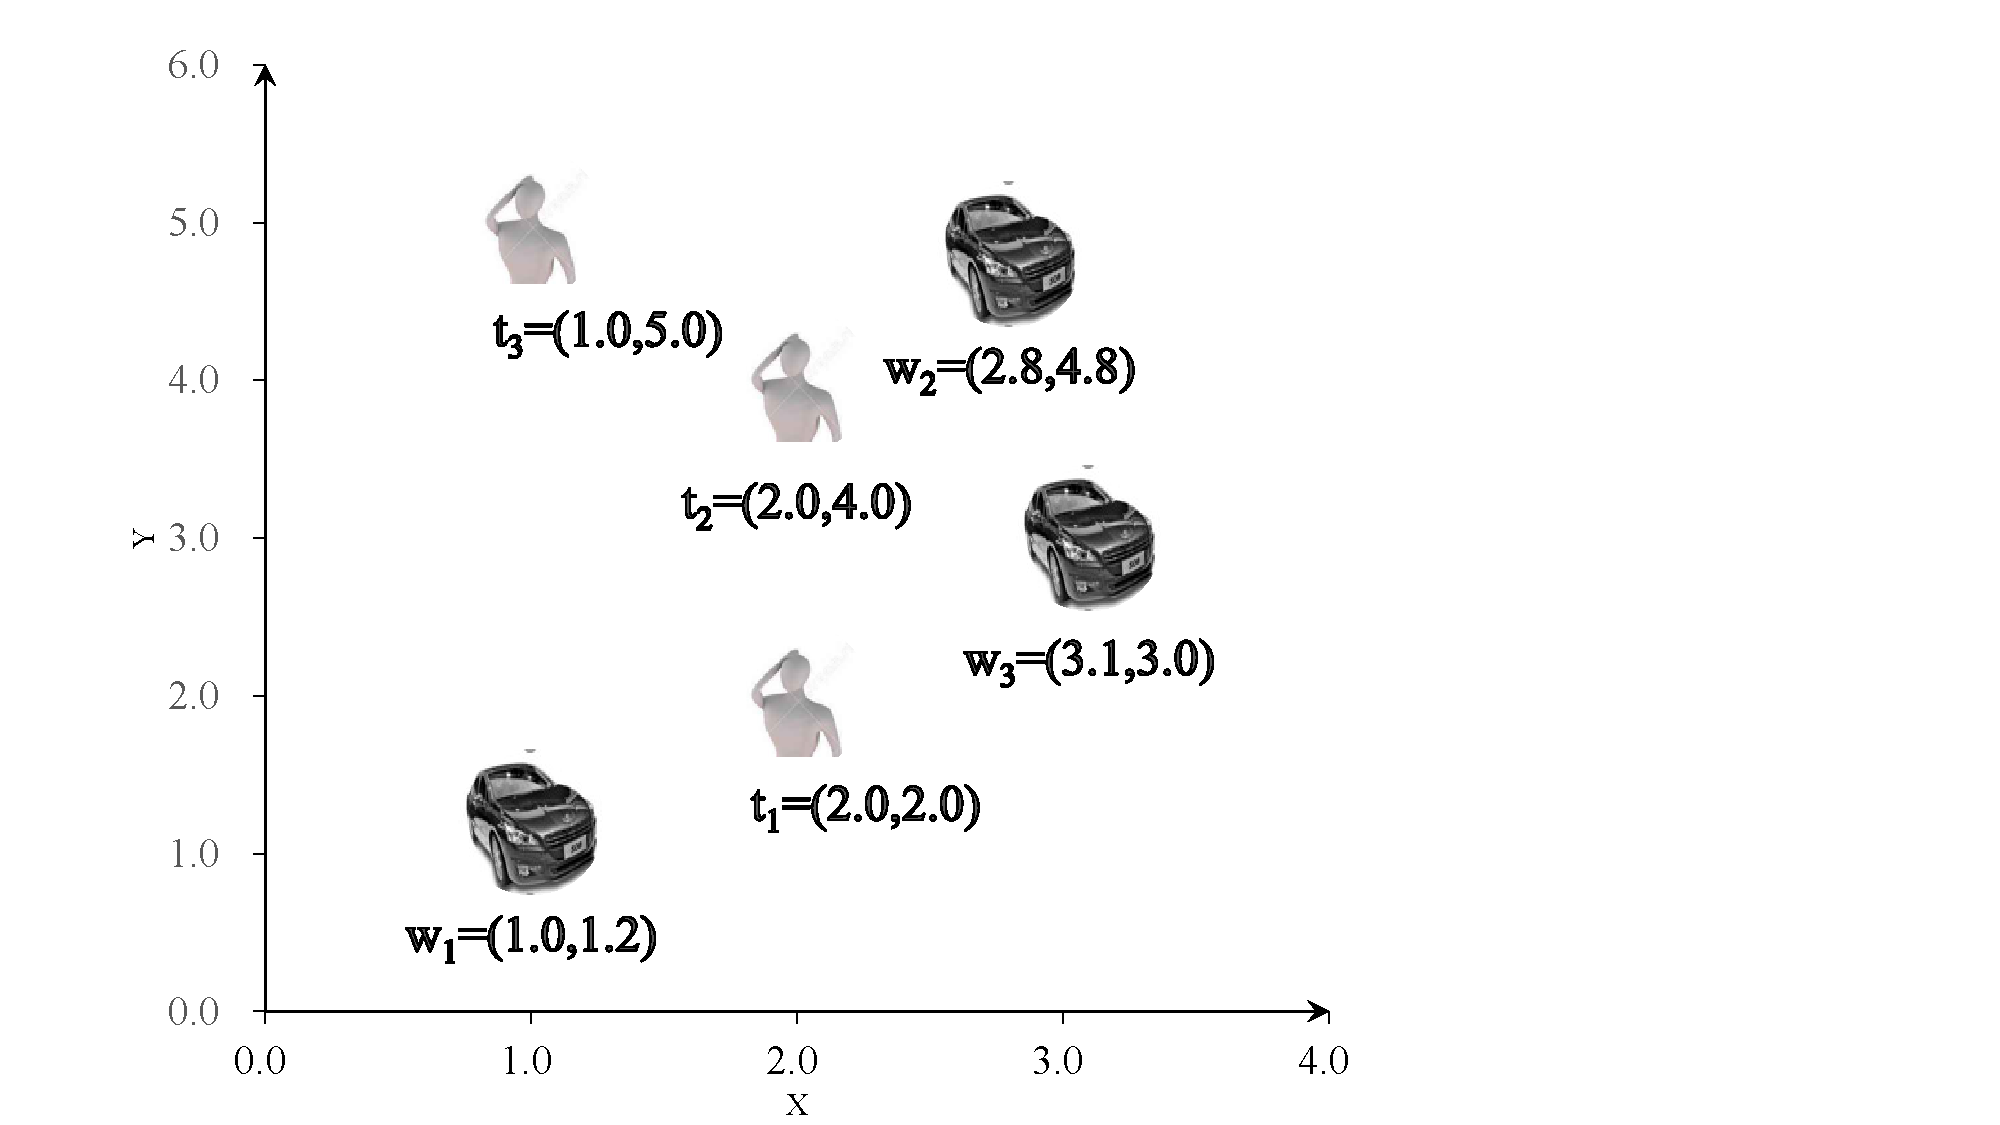
\includegraphics[width=10.5cm]{ex1.pdf}
	\caption{Locations of tasks and workers}
	\label{fig:insert}
\end{figure}

From the example we can see the necessity of a new distance definition. However, what shall we do to work out the matching with the highest revenue? In this paper we adopt a concept called Substitutable\cite{xia2017revenue}, which provides tasks more chances to be matched and performs better with extended distance definition because of an increased number of equal situation. %\cite{xia2017revenue} uses this concept to deal the equal situations when pricing in online labor markets\\

As discussed above, we propose a new problem called {\it Revenue-Maximizing Online Stable Matching (RMOSM)} problem. As indicated in Example 1, overly strict distance definition might cause the loss of revenue. While in the real-world case, passengers care little about assigned drivers' distance varying about 100 meters, which is acceptable. 
%Existing studies\cite{zhao2019preference} only consider the traditional distance definition. 
Thus we redefine the distance as a mapping from euclidean distance to a discrete set and introduce the sustainability concept to create more chances for assignment. We build a new model and propose a new algorithm called {\it Equation-Substitutable Online Matching(ESOM)} to solve the {\it RMOSM} problem. We make the following contribution:
\begin{itemize}
	\item %\TODO{by relaxing the definition of distance we define a new problem called xxx}. 
	{We redefine the distance between workers and tasks from strict Euclidean distance to relaxed distance and propose a new problem called Revenue-Maximizing Online Stable Matching (RMOSM).}
	\item We adopt the concept of  Substitutable\cite{xia2017revenue} to help the system to increase the overall profit of matching by offering more chances to tasks to be assigned with workers.
	\item We propose a new algorithm, Equation-Substitutable Online Matching(ESOM),  which could solve the RMOSM problem to an answer with higher overall profit against the Baseline algorithm, but the running time performs at the same level.
	\item %\TODO{experiments} 
	{We verify the effectiveness and efficiency of the ESOM algorithm with experiments on synthetic and real datasets.}
\end{itemize}
The rest of the paper is organized as follows. In section 2, some works related to our problem are discussed. In Section 3, we introduce some basic definitions and formulate the problem, then put forward a baseline algorithm to deal with the problem. In Section 4, we present another algorithm ESOM with the new concept Substitutable. In Section 5, in the experiments we compare two algorithms' performance under different factors and show ESOM's advantage to the baseline algorithm. We finally conclude this paper in Section 6.


\section{Related Work}

\noindent Our problem can be viewed as the online version of Stable Marriage\cite{gale1962college}, which is a combination of stable marriage problem and online matching problem, and we consult some related work as follow.

\textbf{Stable Marriage}. The stable marriage problem is firstly introduced in \cite{gale1962college}, in which proposes some classic concepts like Stable. Since then, this matching model has been applied to lots of situations\cite{gusfield1989stable,david2013algorithmics}. In heterogeneous distributed systems, the concept of stability is used to balance the efficiency and user satisfaction for optimality\cite{lee1999online}. Some consider optimizing the choice when matching, like using the concept of Substitutable \cite{deng2017complexity,xia2017revenue}. This concept's application offers objects more possibility to be matched from the overall perspective. However, the limit of a feasible matching number exists as before. Similar to our problem, 
the online stable matching problem is studied in \cite{khuller1994line,lee1999online}. In \cite{khuller1994line}, it brings out an on-line weighted bipartite matching problem as an online stable marriage model. As for crowdsourcing, \cite{xia2017revenue} considers pricing and revenue-maximizing towards the stable marriage-like problem, and it also uses the concept of Substituatable,  while \cite{xia2017revenue} focuses mainly on pricing and maximizing revenue. Besides, some effort was made on house-roommates stable matching to maximize the social welfare \cite{huzhang2017online}.

\textbf{Online Matching}. 
The RMOSM problem is an online stable matching problem, which can be regarded as the online version of specified stable marriage\cite{gale1962college}. The input of RMOSM is a bipartite graph $G=(U,V,E)$, where $U$ represents the offline set of workers while $V$ represents the online set of tasks. Once a $v \in V$ arrives, the edges $(u,v) \in E$ incident to $v$ are revealed. The goal of the RMOSM  problem is to maximize the overall profit from the matched tasks. At the same time, an online matching platform needs some principle to keep impartial when matching like the stable concept from offline stable marriage problem\cite{gale1962college}.

Batch-based Solution\cite{kazemi2012geocrowd} is a classic method to reduce the online scenario to an offline scenario. The basic idea of batch based solution is to periodically match tasks with workers in the static scenario\cite{kazemi2012geocrowd,DBLP:conf/gis/KazemiSC13}. It fixes one time stamp and deals with all the existing tasks as an offline problem to work out a local assignment and remove the matched ones from the corresponding sets. For every time step the batch mode will solve a local assignment out, and if we assume an end of time axis, the final matching set is just the combination of all the former local matching sets. As reduced to offline problem, the original problem is feasible and possible to be dealt with wildly-used methods on the offline stable matching \cite{gale1962college}. Kazemi uses the technique to deal with maximum task assignment (MTA)\cite{kazemi2012geocrowd,DBLP:conf/gis/KazemiSC13}. Heterogeneous distributed systems\cite{lee1999online} uses batch mode to simplify the dynamic data sets. And it plays a vital role in dynamic spatial crowdsourcing \cite{DBLP:journals/sigspatial/TongZ18,Tong2019,DBLP:conf/icde/WangTLXXL19,DBLP:conf/icde/ZengTCZ18,tongTKDE19}.

\section{Problem Statement}

\noindent In this section we will introduce the basic concepts and definition of the Revenue-Maximizing Online Stable Matching(RMOSM) Problem, and a baseline approach to deal with the RMOSM problem.

\subsection{Preliminaries and Definition} 

\textbf{Definition 1 (Task)}. {\it A task, denoted by 
	\begin{equation}
	t=< l_t,s_t,d_t,p_t >
	\end{equation}
	released on the platform at time $s_t$ and at location $l_t$ in the 2D space, needs to be served with a delivery worth $p_t$ within $d_t$ time. In other words, the task $t$ will leave from the platform if it's not assigned to a worker before the time $s_t+d_t$.}

\textbf{Definition 2 (Worker)}. {\it A worker, denoted by 
	\begin{equation}
	w = <l_w,s_w,t_w>
	\end{equation}
	appears on the platform with an initial location $l_w$ in the 2D space at time $s_w$, and only accepts the task to which the distance from the worker is no more than $t_w$. In other words, if there is a task $r$ and the distance between $r$ and $w$ is more than $t_w$, r cannot be assigned to w in any instance.}

Normally, a task request is often put forward with a destination rather than the travel cost, which is easy to calculate with the starting point and the destination. in the 2D space. We assume that workers only consider the travel cost related to the tasks, and then the travel costs serve as the same role as the travel distance to workers, simplifying the following discussion.

\textbf{Definition 3 (Distance)}. {\it The distance, denoted by d(t,w), depends on a certain mapping from $T \times W$ to $R$, which can be defined as 
	\begin{equation}
	d(t,w) = \lfloor (|t-w|)/\delta \rfloor \times \delta
	\end{equation}
	and the $\delta$ is a given parameter. }

Note that we don't define the distance simply as Euclidean Distance but a relaxed distance. For example, the Euclidean Distance($d_1$) between $w_1$ and $t_1$ is 11.0, while that($d_2$) between $w_2$ and $t_2$ is 11.2, which is different from the former one. But as for our distance definition, it's possible that $d(t_1,w_1)$ and $d(t_2,w_2)$ are both classified to one batch denoted 11. Because in most situations, the passengers do not care about the little difference between 11.0 and 11.2, and ignoring the difference horizons the set of {\it stable matching}, which benefits to possibly improve the overall profit.

\textbf{Definition 4 (Matching)}. {\it Given a set of tasks T and a set of workers W, a matching, denoted by M $\in$ T $\times$ W, insists of binary pairs  $< t, w >$. Certain t or w don't appear twice in different pairs.}


\textbf{Definition 5 (Blocking Pair)}. {\it A blocking pair, denoted by $< t, w >$ $\in$ T $\times$ W, satisfies following condition:
	
	There is another pair $< t^ *, w^ * >$, and
	\begin{equation}
	\begin{split}	
	&p_{t^*} < p_t\ or\ w\ is\ unmatched\\
	&d(t,w^*) < d(t,w)\ or\ t\ is\ unmatched\\
	\end{split}
	\end{equation}
}

\textbf{Definition 6 (Stability)}. {\it A matching M is stable if $\forall$ $< t, w >$ $\in$ $T \times W$, $< t, w >$ is not a blocking pair.}

\textbf{Definition 7 (Time Window)}. {\it Given a set of tasks T, a set of workers W and the time window's length h, we denote $min_{t \in T}s_t$ as $h_0$ and [$h_0$, $h_0$ + h) as $H_0$, 
	\begin{equation}
	H_i=[h_i,h_{i+1})=[h_0 + i * h, h_0 + (i + 1) * h),i=1,2,...
	\end{equation}
	In this way we divide the time axis into several periods, which are denoted as time windows. 
}

\textbf{Definition 8 (Revenue)}. {\it Given a matching $M$,the revenue of M is denoted by 
	\begin{equation}
	R = \Sigma_{<t,w>\in M}p_t
	\end{equation}
}

\textbf{Definition 9 (Revenue-Maximizing Online Stable Matching Problem)}. {\it Given a set of tasks T, a set of workers W and time windows $\{h_i\}_{0}^{\infty}$ based on T and W, we define
	\begin{equation}
	T_0=\{t\in T|s_t \in H_0\}
	\end{equation}
	\begin{equation}
	W_0=\{w\in W|s_w \in H_0\}
	\end{equation}
	Our problem begins with $T_0$ and $W_0$. We deal with $T_i$ and $W_i$ to find a stable matching $M_i$, then turn to next time window $H_{i+1}$ for another stable matching problem about $T_{i+1}$ and $W_{i+1}$, and
	\begin{equation}
	T_{i+1}=\{t\in T|s_t<h_{i+1},(s_t+d_t)>h_{i+1},t\ is\ unmatched.\}
	\end{equation}
	\begin{equation}
	W_{i+1}=\{w\in W|s_w<h_{i+1},w\ is\ unmatched.\}
	\end{equation}
	
We get series of stable matching ${M_i}_0^{\infty}$. Then for each $M_i$ we calculate the revenue $R_i$, and for certain fixed normal number n, define overall revenue R as $\Sigma_{i=0}^{n}R_i$. 

The Revenue-Maximizing Online Stable Matching Problem is to find an algorithm that could give a stable matching with revenue as high as possible. 
}

The online platform has a time axis with infinite length, so we fix a number $m$ as the time scale for the convenience of analysis. Then the online problem is divided into $m+1$ offline problems. 

\subsection{A Baseline Approach}
In this section, we'll simply introduce a baseline algorithm Online-Greedy, in which there is a sub-algorithm called Local-Match. The main procedures of those are presented in Algorithm 1 and Algorithm 2.

The idea of the baseline algorithm is based on Chain Algorithm\cite{wong2007efficient,karp1990optimal}. The Chain Algorithm's contribution is to solve a stable matching problem on Euclidean distance metric space about closet pairs. Applied to our problem, though the metric standard differs, the algorithm and the proofs are almost the same. 

For Algorithm 1, in lines 1-4, Online-Greedy divides the time axis into $n$ parts equally, and the length of each part is all set with h. In line 5, the algorithm starts a cycle for each batch. In lines 6-7, at batch $[h_i,h_{i+1})$, we get tasks' and workers' set  $T_i$ and $W_i$ in which members are capable at the recent batch $[h_i,h_{i+1})$. In line 8, by sub-algorithm Local-Match($T_i$,$W_i$), which will be illustrated later, the result of this period is denoted by $M_i$. In lines 9-12, if t $\in T_i$ or w $\in W_i$ appears at certain pair in $M_i$, remove $t$ or $w$ from $T$ or $W$. In line 13, stop this batch and turn to the next one if any. In line 14, with the sub-problem of each divided period solved we get $n$ results $M_0,M_1,...,M_{n-1}$, and $M = \bigcup^{n-1}_{0}M_i$ is our final answer.

As for Algorithm 2 Local-Match, given parameters $T$ and $W$, in line 1, the algorithm firstly initializes the $M$ as an empty set. In lines 2-9, as long as $T$ is not empty, select $t$ from $T$ as who offers the highest price, then set $W_t$ containing all workers in $W$ capable to $t$ and $w$ is the one who is closest to $t$ in $W_t$.In lines 6-8, add pair $(t,w)$ to $M$, then delete $t$ from $T$ and $w$ from $W$, then turn to line 2 for check. When the cycle ends, return $M$ as answer in line 10.

\begin{algorithm}[h]
	\caption{Online-Greedy($T,W,h,n$)}
	\label{alg1}
	\begin{algorithmic}[1]
		\REQUIRE Tasks:$T$, Workers:$W$, Length of steps:$h$, Number of time windows:$n$
		\ENSURE Matching:$M$
		\STATE $h_0 \leftarrow \min_{t \in T}s_t$
		\FOR{$i=1$ to $n$}
		\STATE $h_i \leftarrow h_0 + h \times i$
		\ENDFOR
		\FOR{$i=0$ to $n$}
		\STATE $T_i \leftarrow \{t\in T|s_t < h_i\ and\ (s_t+d_t) > h_i\}$ 
		\STATE $W_i \leftarrow \{w\in W|s_w < h_i\}$
		\STATE $M_i \leftarrow$ Local-Match$(T_i,W_i)$
		\FOR{each $(t,w)$ in $M_i$}
		\STATE Remove $t$ from $T$
		\STATE Remove $w$ from $W$
		\ENDFOR
		\ENDFOR
		\STATE $M \leftarrow \bigcup_{0}^{n-1} M_i$
		\RETURN $M$	
	\end{algorithmic} 
\end{algorithm}


\begin{algorithm}[h]
	\caption{Local-Match($T,W$)}
	\label{alg2}
	\begin{algorithmic}[1]
		\REQUIRE Tasks:$T$, Workers:$W$
		\ENSURE Matching:$M$
		\STATE $M \leftarrow \emptyset$
		\WHILE{$T\neq \emptyset$}
		\STATE $t \leftarrow argmax_{t\in T}p_t$
		\STATE $W_t \leftarrow \{w\in W|d(t,w)\leq t_w\}$
		\STATE $w \leftarrow argmin_{w\in W_t}d(t,w)$
		\STATE Assert $(t,w)$ into $M$
		\STATE Remove $t$ from $T$
		\STATE Remove $w$ from $W$
		\ENDWHILE
		\RETURN $M$
	\end{algorithmic} 
\end{algorithm}

%\begin{figure}[ht]
%	\centering
%	\includegraphics[width=8.5cm]{mex2.pdf}
%	\caption{Exmaple 2}
%	\label{fig:insert}
%\end{figure}

\textbf{Example 2}. We have 3 tasks $t_1 - t_3$ and 3 workers $w_1-w_3$ on certain taxi-dispatching platform, whose attributes are listed in TABLE 1 and TABLE 2, while locations are shown in Figure 1. Here the distance between $t$ and $w$ is defined as follows: $d(t,w)=\lfloor (|t-w|)/\delta \rfloor \times \delta$. Here the $\lfloor x \rfloor$ is the integer part of $x$, $|t-w|$ is the strict euclidean distance between $t$ and $w$ while $\delta$ is a fixed given parameter which is set as 0.5 in this example. And [0,1] is set as the first time window, (1,2] is set as the second one. With algorithm Online-Greedy, in the first time window, {$t_1$} and {$w_1$,$w_2$,$w_3$} are dealt with Local-Match, And the matching starts from $t_1$. Due to the existence of the threshold, only $w_1$ and $w_3$ are available for $t_1$, and $w_1$ is assigned to $t_1$ because of its order. We add pair $(t_1,w_1)$ to $M_1$, then turn to the second time window. As the price of $t_2$ ranks first, we assign $w_2$ to $t_2$ for the order and add $(t_2,2_2)$ to $M_2$. While there are only $t_2$ and $w_3$ left but they are not able to be matched for threshold. Thus, our algorithm ends with result $M = M_1 \bigcup M_2 = \{(t_1,w_1),(t_2,w_2)\}$, and the revenue is 7.

\textbf{Complexity Analysis}. For each time window, the time complexity of the baseline is $O(|T_i||W_i|)$. As the largest number of time windows that one task covers is generally limited to a finite constant, with given $T$ and $W$ for the whole time period, the time complexity is  $O(|T||W|)$.

However, as the result set is enlarged by relaxed distance, Online-Greedy algorithm has the problem with solving out the result closer to the optimal one. In example 1 we analyze the possible matching of the given problem, and the best matching is $M^{'}$ with revenue 9, while the baseline algorithm's answer is only 7. It's because that Online-Greedy's strategy on selecting towards equal distance performs badly so that it's unable to find the optimal result. 

In example 2, if $t_2$ is assigned to $w_3$ instead of $w_2$, as $d(t_2,w_3)=d(t_2,w_2)$, $t_3$ will be matched successfully with $w_2$ rather than remains unmatched, which increases the revenue of final matching directly. It's the shortcoming of the Online-Greedy algorithm.

Thus, we ought to design a new algorithm with a new feature to deal with the equation situation properly.


\section{ESOM Algorithm}

\noindent In this section, we present an overview of a new algorithm to deal with the Revenue-Maximizing Online Stable Matching problem(RMOSM) problem. As shown in the Baseline Approach, tasks are sorted in the order of price for matching. Therefore, the revenue of the taxi-dispatching platform is directly proportional to the number of matched pairs. Following this feature, to improve the Greedy algorithm, we focus more on how to increase the possibility of tasks to be matched.

Note that the attribute $t_w$ of $w$, which represents the threshold, entails a possible consequence: during one matching in which $p_{t_1} < p_{t_2}$, only $t_1$ is available to be matched. The following Example 3 shows one kind of instance that threshold makes sense in matching causing the former described situation.

From example 2 we can see Online-Greedy has shortcomings so we get $\{(t_1,w_1),(t_2,w_3)\}$ rather than $\{(t_1,w_2),(t_2,w_1),(t_3,w_3)\}$ as results to gain higher profit. To increase the possibility of tasks to be matched, we introduce a new concept called Substitutable.

\textbf{Definition 10 (Substitutable)\cite{xia2017revenue}}. {\it Given a matching $M$ and matched pair $(t,w)$ $\in$ $M$, worker $w$ is substitutable if there exits an unmatched worker $w^{'}$ that $d(t,w)=d(t,w^{'})$.
}

This concept is presented in \cite{xia2017revenue} to deal with a pricing problem about matching. Algorithm 3 and Algorithm 4 illustrate the procedure of the Equation-Substitutable Online Matching algorithm, simplified as ESOM algorithm.

The ESOM algorithm is based on traditional methods for stable matching like the Gale-Shapley algorithm or Chain algorithm, and it reduces the online scenario to the offline scenario by a batch-based solution. For the relaxed distance applied to our model, when a passenger appears on the platform, the drivers closest to him consist of a non-single set. In this way, the Substitutable concept offers workers more chances to be matched when distance's equation happens and helps to increase the number of matched pairs.

\begin{algorithm}[h]
	\caption{ESOM($T,W,h,n$)}
	\label{alg3}
	\begin{algorithmic}[1]
		\REQUIRE Tasks:$T$, Workers:$W$, Length of steps:$h$, Number of time windows:$n$
		\ENSURE Matching:$M$
		\STATE $h_0 \leftarrow \min_{t \in T}s_t$
		\FOR{$i=1$ to $n$}
		\STATE $h_i \leftarrow h_0 + h \times i$
		\ENDFOR
		
		\FOR{$i=0$ to $n$}
		\STATE $T_i \leftarrow \{t\in T|s_t < h_i\ and\ (s_t+d_t) > h_i\}$ 
		\STATE $W_i \leftarrow \{w\in W|s_w < h_i\}$
		\FOR{each $t$ in $T_i$}
		\STATE $r_t \leftarrow 0$
		\ENDFOR
		\STATE $M_i = LE(T_i,W_i)$
		\FOR{each $(t,w)$ in $M_i$}
		\STATE Remove $t$ from $T$
		\STATE Remove $w$ from $W$
		\ENDFOR
		\ENDFOR
		\STATE $M \leftarrow \bigcup_{0}^{n-1} M_i$
		\RETURN $M$	
	\end{algorithmic} 
\end{algorithm}

For Algorithm 3, in lines 1-4, ESOM divides the time axis into $n$ parts equally, and the length of each part is all set with $h$. In line 5, the algorithm starts a cycle for each batch. In lines 6-7, at batch $[h_i,h_{i+1})$, we get tasks' and workers' sets  $T_i$ and $W_i$ in which members are capable at recent batch $[h_i,h_{i+1})$. While in lines 8-10, we set an attribute $r_t$ of $t$ as 0, for each $t \in T_i$, which is representative of whether $t$ has failed in ever matching or not, because passengers sometimes might find no drivers available on the recent platform. In line 11, by sub-algorithm LE($T_i$,$W_i$), which will be illustrated later, the result of this period is denoted by $M_i$. In lines 12-14, if $t$ $\in T_i$ or $w$ $\in W_i$ appears at certain pair in $M_i$, we remove $t$ or $w$ from $T$ or $W$. In line 16, we stop this batch and turn to the next one if any. In line 17, with sub-problem of each divided period solved out we get $n$ results $M_0,M_1,...,M_{n-1}$, and $M = \bigcup^{n-1}_{0}M_i$ is our final answer.

\begin{algorithm}[h]
	\caption{LE($T_i,W_i$)}
	\label{alg4}
	\begin{algorithmic}[1]
		\REQUIRE Tasks:$T_i$, Workers:$W_i$
		\ENSURE Matching:$M_i$
		\STATE $M_i \leftarrow \emptyset$
		\WHILE{$T_i \neq \emptyset$}
		\STATE $t \leftarrow argmax_{t\in T_i}p_t$
		
		\STATE $W_t \leftarrow \{w\in W|d(t,w)\leq t_w\}$		
		\STATE $M_i,T_i,W_i,W_t = SC(M_i,T_i,W_i,W_t,t)$
		\IF{task $t$ is unmatched}
		\IF{$r_t=0$} 
		\STATE $r_t \leftarrow 1$
		\STATE Reset $W_t$
		\ENDIF
		\ELSE
		\STATE Remove $t$ from $T_i$
		\ENDIF
		\ENDWHILE	
		\RETURN $M_i$
	\end{algorithmic} 
\end{algorithm}

For Algorithm 4, given parameters $T_i$ and $W_i$, in line 1, the algorithm firstly initializes the $M_i$ as an empty set. In lines 2-14, if $T_i$ is not empty, and in line 3, we select $t$ from $T_i$ as who offers the highest price. In line 4 we set $W_t$ in which workers can accept the task, and in line 5 another sub-algorithm SC is performed. In line 6, we check if $t$ is not matched. If so, in lines 7-10, when $r_t$ = 0, set it as 1 and reset $W_t$, which means $t$ is gifted with another chance to be matched and takes priority from a certain perspective. In line 9, we reset $W_t$ for another matching of $t$; if not, we remove $t$ from $T_i$ and $t$ loses its matching chance at this batch. Until $T_i$ is empty, in line 15, the algorithm returns $M_i$ as this batch's answer set.

\begin{algorithm}[h]
	\caption{SC($M_i,T_i,W_i,t$)}
	\label{alg5}
	\begin{algorithmic}[1]
		\REQUIRE Matching:$M_i$, Tasks:$T_i$, Workers:$W_i$, Available Workers:$W_t$,Task:$t$
		\ENSURE Matching:$M_i$, Tasks:$T_i$, Workers:$W_i$, Available Workers:$W_t$
		\WHILE{$W_t\neq \emptyset$ and t is unmatched}
		\STATE $w \leftarrow argmin_{w\in W_t}d(t,w)$
		\IF{$w$ is unmatched}
		\STATE Assert $(t,w)$ into $M_i$
		\STATE Remove $w$ from $W_t$
		\ELSE
		\STATE (Assume $w$ was assigned to $t^{'}$)
		\IF{$w$ is substitutable}
		\STATE Replace $(t^{'},w)$ in $M_i$ with $(t,w)$
		\STATE Replace $t$ in $T_i$ with $t^{'}$
		\IF{$p_{t^{'}}=p_t$ and $r_{t^{'}}<r_t$}
		\STATE Remove $w$ from $W_{t^{'}}$
		\ENDIF
		\ELSE 
		\STATE Remove $w$ form $W_t$
		\ENDIF
		\ENDIF
		\ENDWHILE
		\RETURN $M_i,T_i,W_i,W_t$
	\end{algorithmic} 
\end{algorithm}

For Algorithm 5, given parameters $M_i$,$T_i$ and $W_i$, in line 1, if $W_i$ is not empty and $t$ is not matched, the algorithm runs lines 2-17. In line 2, select $w$ from $W_t$ as who is nearest to $t$. In lines 3-5, if $w$ is unmatched, add $(t,w)$ to $M_i$ and remove $w$ from $W_t$; if not, we assume $w$ was assigned to $t^{'}$ before. In line 8, we judge whether $w$ is substitutable, and if so, rematch $w$ with $t$ rather than $t^{'}$ and replace $t$ in $T_i$ with $t^{'}$, then in line 11, if the price of $t^{'}$ and $t$ is equal while $r_{t^{'}} < r_t$, we remove $w$ from $W_{t^{'}}$; if not, we remove $w$ from $W_t$. After finishing above, in line 17, we turn back to line 1 for the next round. When the cycle ends, return $M_i$,$T_i$ and $W_i$ as answers.

\begin{figure*}[htb]
	\centering
	\subfigure[Utility, run time and memory of varying $|T|$ ($|W|$ = $|T|$)]{
		\label{fig:subfig:a} %% label for first subfigure	
		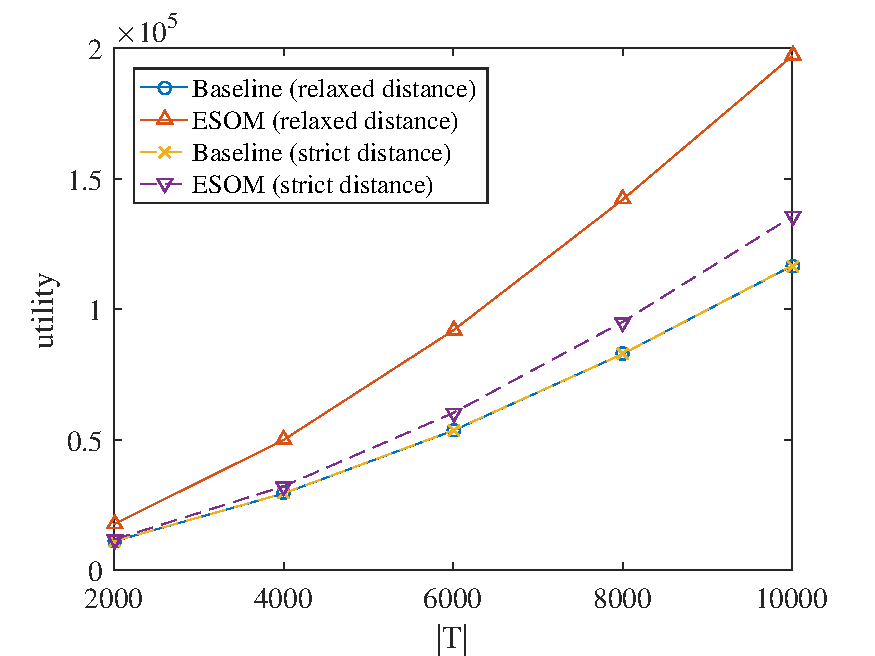
\includegraphics[height=0.18\textheight,width=0.31\textwidth]{f2.pdf}
		\label{fig:subfig:a} %% label for first subfigure	
		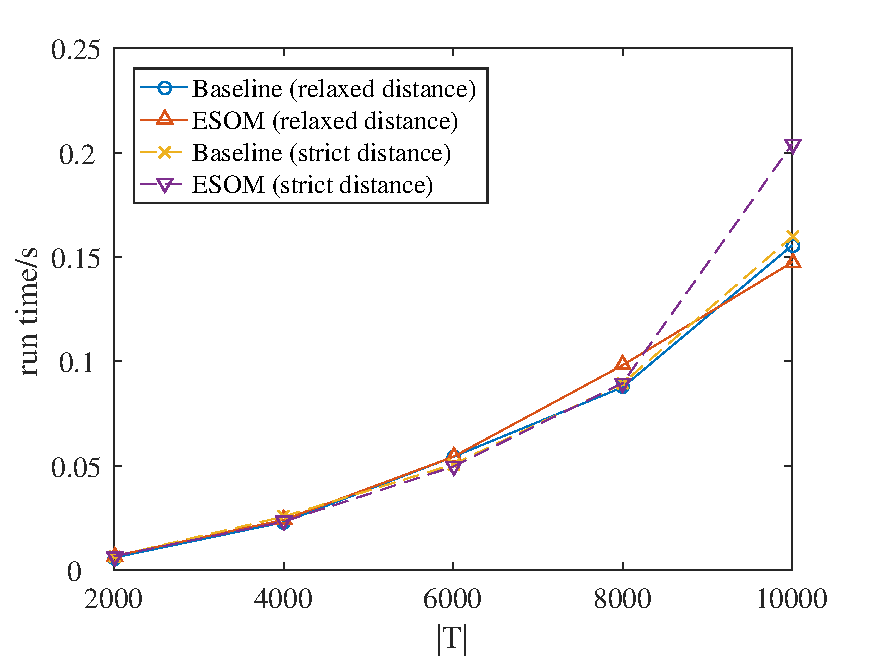
\includegraphics[height=0.18\textheight,width=0.31\textwidth]{f3.pdf}
		\label{fig:subfig:a} %% label for first subfigure	
		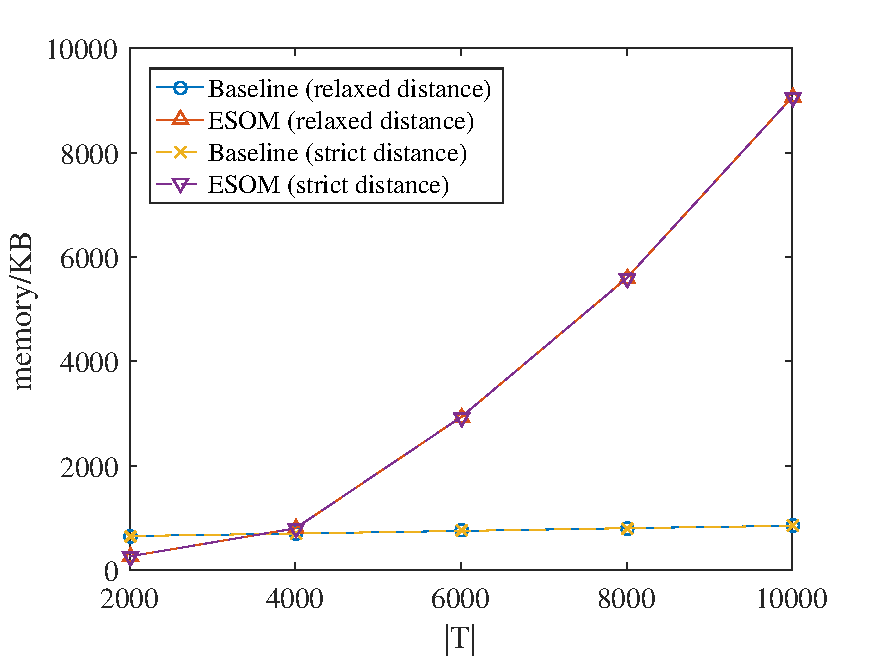
\includegraphics[height=0.18\textheight,width=0.31\textwidth]{f4.pdf}}
	\hspace{1in}
	~~	
	\subfigure[Utility, run time and memory of varying $|T|$]{	
		\label{fig:subfig:b} %% label for second subfigure	
		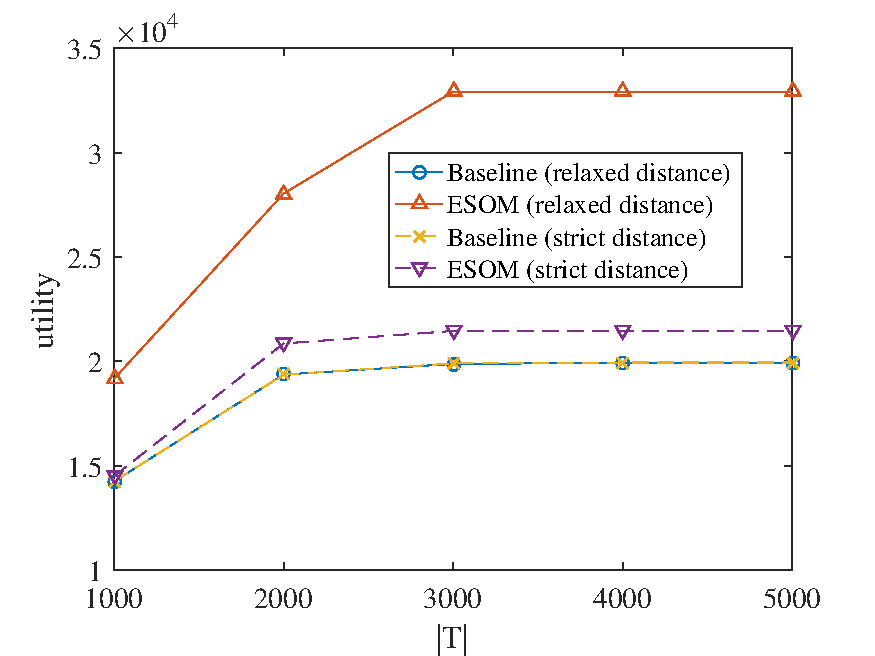
\includegraphics[height=0.18\textheight,width=0.31\textwidth]{f5.pdf}
		\label{fig:subfig:b} %% label for second subfigure	
		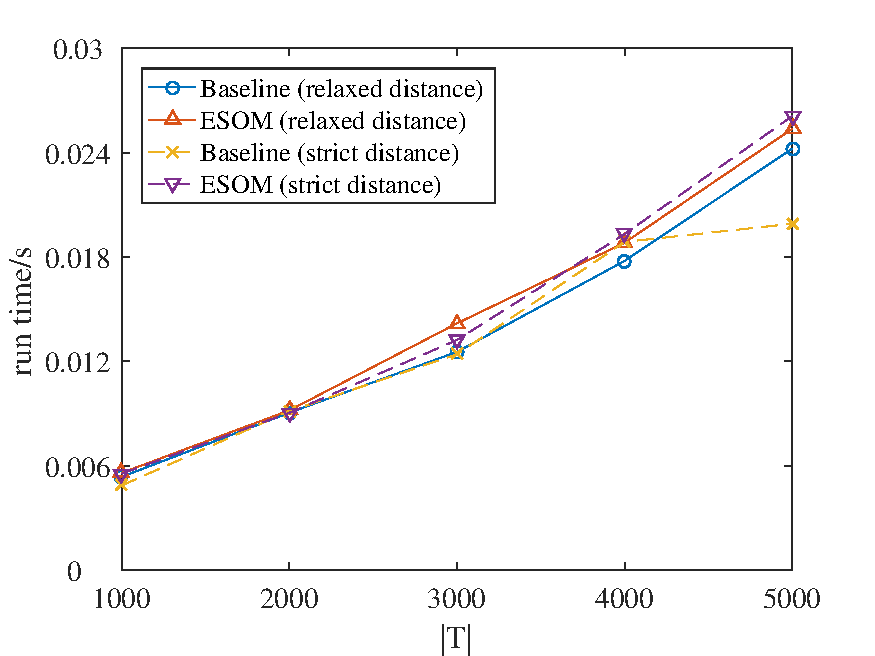
\includegraphics[height=0.18\textheight,width=0.31\textwidth]{f6.pdf}
		\label{fig:subfig:b} %% label for second subfigure	
		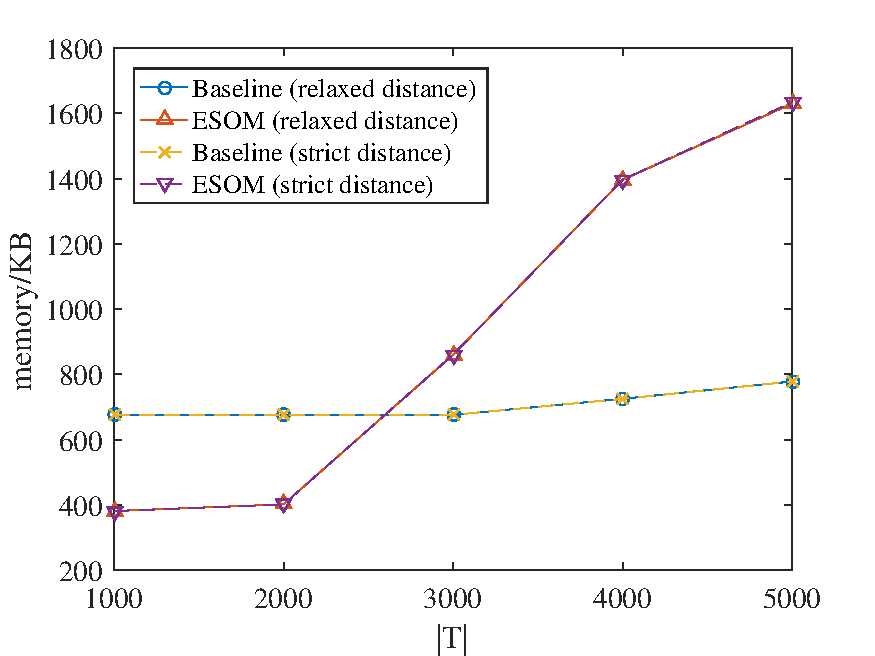
\includegraphics[height=0.18\textheight,width=0.31\textwidth]{f7.pdf}}
	\hspace{1in}
	~~	
	\subfigure[Utility, run time and memory of varying $|W|$]{
		\label{fig:subfig:a} %% label for first subfigure	
		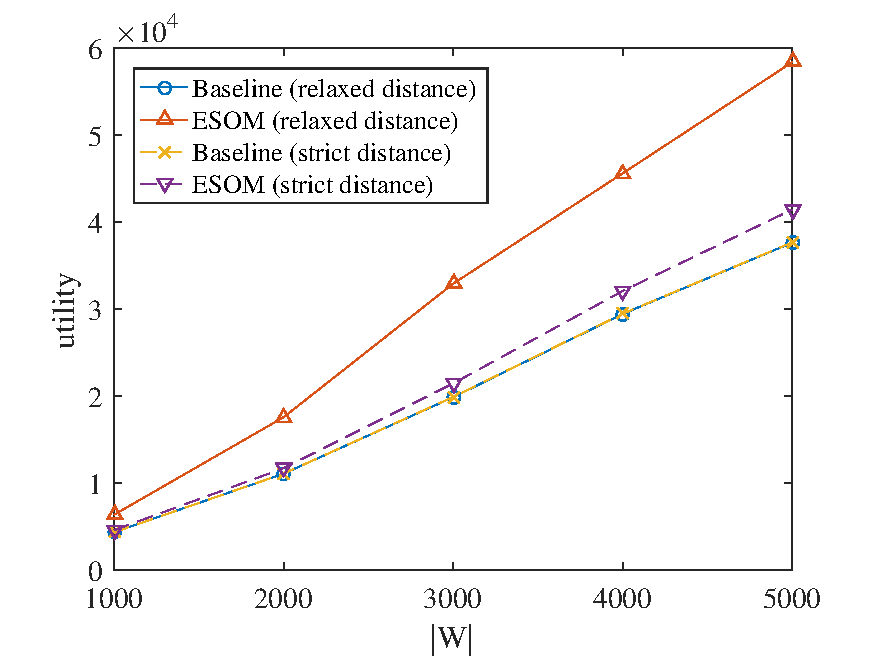
\includegraphics[height=0.18\textheight,width=0.31\textwidth]{f8.pdf}
		\label{fig:subfig:a} %% label for first subfigure	
		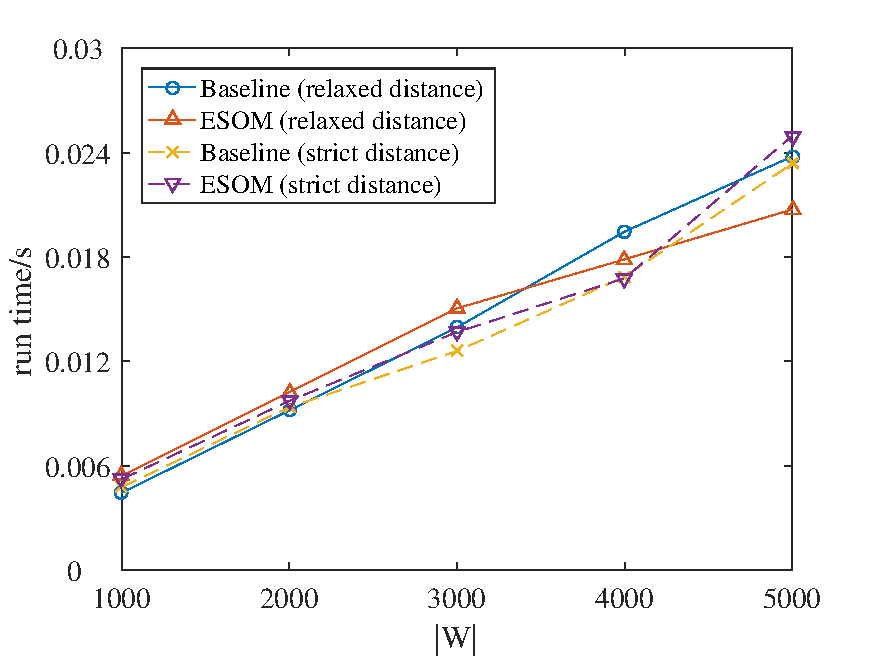
\includegraphics[height=0.18\textheight,width=0.31\textwidth]{f9.pdf}
		\label{fig:subfig:a} %% label for first subfigure	
		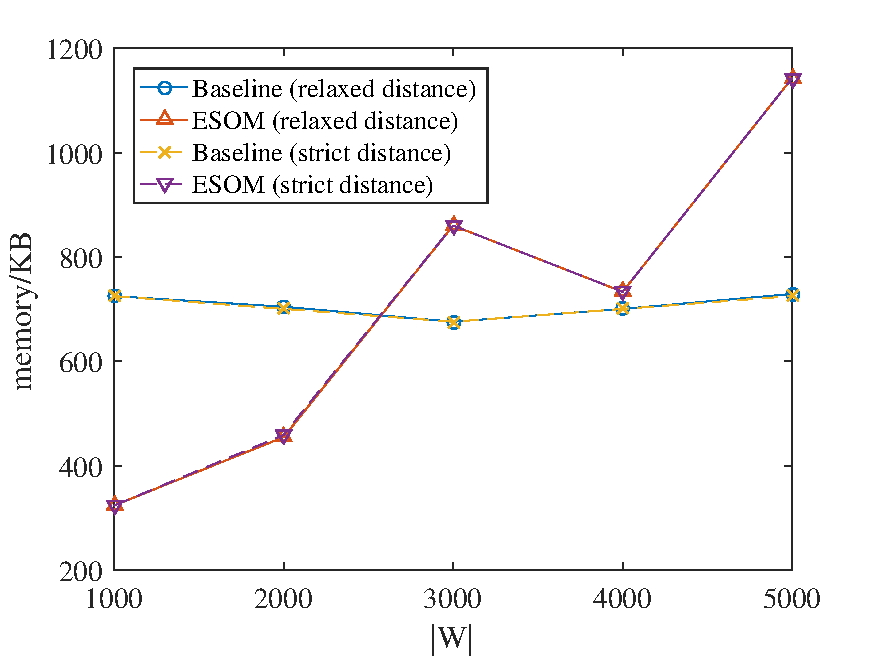
\includegraphics[height=0.18\textheight,width=0.31\textwidth]{f10.pdf}}
	\hspace{1in}
	~~	
	\caption{Results on varying $|T|$ and $|W|$}
	\label{fig:subfig} %% label for entire figure
\end{figure*}



\textbf{Example 3}. We have 3 tasks $t_1 - t_3$ and 3 workers $w_1-w_3$ on the certain taxi-dispatching platform, whose attributes are listed in TABLE 1 and TABLE 2, while locations are shown in Figure 1. Here the distance between $t$ and $w$ is defined as follows: $d(t,w)=\lfloor (|t-w|)/\delta \rfloor \times \delta$. Here the $\lfloor x \rfloor$ is the integer part of $x$, $|t-w|$ is the strict euclidean distance between $t$ and $w$ while $\delta$ is a fixed given parameter which is set as 0.5 in this example. And [0,1] is set as the first time window, (1,2] is set as the second one. With algorithm ESOM, in the first time window, {$t_1$} and {$w_1$,$w_2$,$w_3$} are dealt with LE, And the matching starts from $t_1$. Due to the existence of the threshold, only $w_1$ and $w_3$ are available for $t_1$, and $w_1$ is assigned to $t_1$ because of its order. We add pair $(t_1,w_1)$ to $M_1$, then turn to the second time window. As the price of $t_2$ ranks first, we assign $w_2$ to $t_2$ for the order and add $(t_2,2_2)$ to $M_2$. There are only $t_3$ and $w_3$ left but they are not able to be matched for the threshold. However, we find that $w_2$ is substitutable because of $w_3$, so we rematch $w_2$ with $t_3$. Then we turn back to $t_2$ and the only choice is to assign $w_3$ to $t_2$. So $M_2 = \{(t_2,w_3),(t_3,w_2)\}$. Thus our algorithm ends with result $M = M_1 \bigcup M_2 = \{(t_1,w_1),(t_2,w_3),(t_3,w_2)\}$, and the revenue is 9.

\textbf{Theorem 1}. {\it Replacing a substitutable worker in a pair with another corresponding worker keeps the whole assignment's stability.}

{\it Proof}. Given a matching set $M$ which is stable, we replace $(t,w) \in M$ with $(t,w')$, where $d(t,w) = d(t,w')$, that is $w$ is substitutable towards $w'$. Then we get a new set $M'$. In $M'$, the only new pair compared to $M$ is $(t,w')$, so it only needs to check whether $(t,w')$ is a blocking pair or not. As $d(t,w) = d(t,w')$, $(t,w')$ is judged as a blocking pair if and only if so do $(t,w)$. While $M$ including $(t,w)$ is stable, $M'$'s stability is preserved after replacing substitutable workers.

\textbf{Complexity Analysis}. For each time window, the time complexity of the ESOM algorithm is $O(|T_i||W_i|)$. As the largest number of time windows that one task covers is generally limited to a finite constant, with given $T$ and $W$ for the whole time period, the time complexity is $O(|T||W|)$.

{\it Proof}. In the time window $H_i$, in algorithm LE($T_i,W_i)$, for each task in $T_i$, SC($M_i,T_i,W_i,W_t,W_t,t$) is implemented. So the number of tasks is $O(|T_i|)$. In the SC algorithm towards one task $t_i$, for each worker in $W_t$, the states of matching and substitutability are checked, so the number of workers is $O(|W_i|)$. Therefore, the time complexity to run a time window of ESOM is $O(|T_i||W_i|)$. As the number of batches is a fix constant $n$, the time complexity of ESOM is $O(|T||W|)$.

\textbf{Definition 10 (Competitive Ratio)}. {\it Suppose there is an online maximization problem, and ALG is a certain algorithm for the problem. We denote the expected performance of ALG on an input $\mathcal{L}$ as $ALG(\mathcal{L})=\mathbb{E}_{\mathcal{I} \sim \mathcal{L}}[ALG(\mathcal{I})]$, in which the $\mathcal{I}$ is a random arrival sequence. Let $OPT(\mathcal{L})=\mathbb{E}[OPT(\mathcal{I})]$ denote the expected offline optimal algorithm, where $OPT(\mathcal{L})$ refers to the optimal value with observed full arrival sequence $\mathcal{I}$. Competitive ratio is defined as $min_{\mathcal{L}}\frac{ALG(\mathcal{L}}{OPT(\mathcal{L})}$.
}

In the RMOSM problem, we simplify the competitive ratio as $\frac{M}{M^{*}}$, where $M$ is the result of the ESOM algorithm, and $M^{*}$ is the optimal result. 

\textbf{Lemma 2}. {\it For each time window, the ESOM algorithm outputs $M$ such that $|M| \geq \frac{2}{3}|M^*|$, where $M^*$ is the matching with optimal profit.}

{\it Proof}. With both $M$ and $M^*$ known exactly, we construct a graph as follows. Set a task node at the graph if and only if the task is matched in either $M$ or $M^*$, similarly for worker nodes. For any certain pair of a task node and a worker node at the graph, if they are matched in $M$, we introduce an undirected edge between them, and if they are matched in $M^*$, similarly introduce an extra undirected edge. It's obvious that each connected component in the graph is either a cycle or path.
For a cycle, it means a common matched pair of both $M$ and $M^*$, so there is no loss for the number of matched pairs. While for a path, as one task or worker can't be matched twice or more in certain matching, a path with even number($2k$) edges consists of $k$ matched pairs from $M$ and another $k$ pairs from $M^*$, which also causes no loss. A path with an odd number($2k+1$) of edges is called an augmenting path. In an augmenting path, matched pairs' numbers of $M$ and $M^*$ are $k$ and $k+1$. Thus, if we prove that the graph doesn't contain augmenting paths with 1 or 3 edges then the lemma is proved naturally.

First, if there exists an augmenting path with only 1 edge(from $M^*$), the task and worker of the path is a blocking pair in $M$, which contradicts with the stability.

Secondly, suppose there exists an augmenting path with 3 edges($<w_1,t_1>,<w_2,t_2>$ from $M^*$, $<t_1,w_2>$ from $M$), for $p_{t_1}$ and $p_{t_2}$, if $p_{t_1} < p_{t_2}$, $<t_2,w_2>$ is a blocking pair in $M$. So $p_{t_1} \geq p_{t_2}$. If $p_{t_1} = p_{t_2}$, as $t_2$ is not assigned to $w_2$ in $M$, $r_{t_1}$ should be 1, but $w_1$ is not matched, 
which contradicts with $r_{t_1}=1$, so $p_{t_1} > p_{t_2}$; For $d(t_1,w_1)$ and $d(t_2,w_2)$, it's easy to see that $d(t_1,w_1) \geq d(t_1,w_2)$, otherwise $<t_1,w_1>$ is a blocking pair in $M$. If $d(t_1,w_1) = d(t_1,w_2)$, $w_2$ is substitutable, it contradicts with that $t_2$ is unmatched.
So $d(t_1,w_1) > d(t_2,w_2)$. However, now $<t_1,w_2>$ is a blocking pair in $M^*$. Therefore augmenting path with 3 edges can't exist. The lemma has been proved.

\textbf{Theorem 3}. {\it For each time window, the profit R resulted from the ESOM algorithm satisfies that $R \geq \frac{2}{3}R^*$, where $R$ is the optimal profit.}

As in ESOM algorithm tasks with higher price have higher priority to be matched, the lemma 2 about the number of matched pairs easily support Theorem 3. Thus, the competitive ratio is $\frac{2}{3}$.

\section{Experimental Study}

\noindent{\it A. Experimental Setup}

\begin{figure*}[htb]
	\centering
	\subfigure[Utility, run time and memory of varying $\alpha$]{
		\label{fig:subfig:a} %% label for first subfigure	
		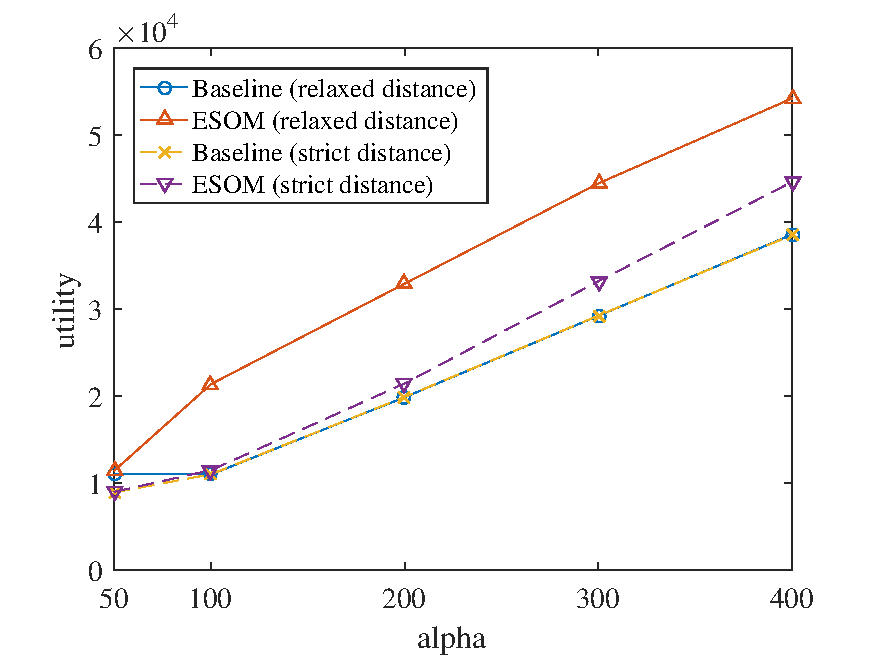
\includegraphics[height=0.18\textheight,width=0.31\textwidth]{f11.pdf}
		\label{fig:subfig:a} %% label for first subfigure	
		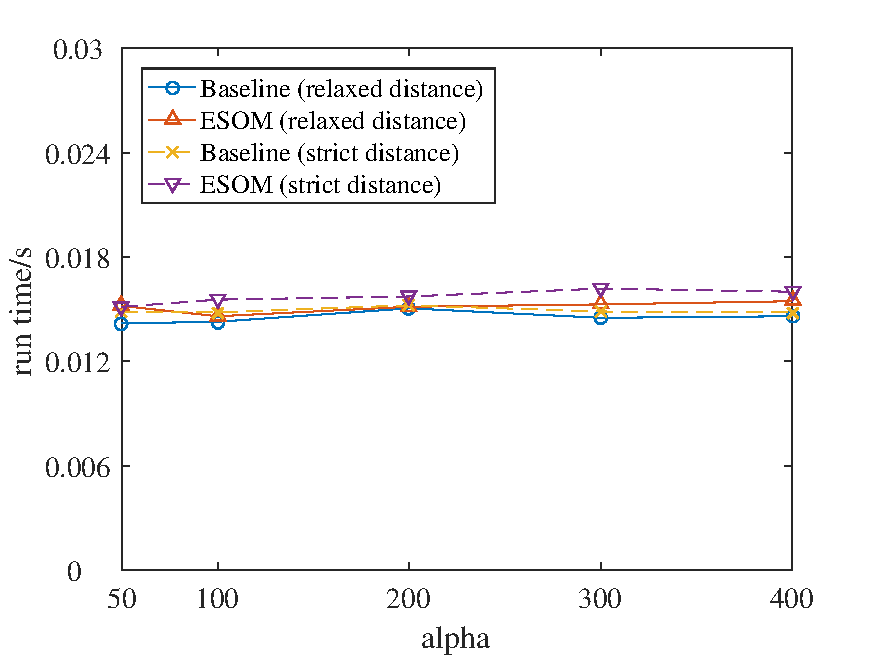
\includegraphics[height=0.18\textheight,width=0.31\textwidth]{f12.pdf}
		\label{fig:subfig:a} %% label for first subfigure	
		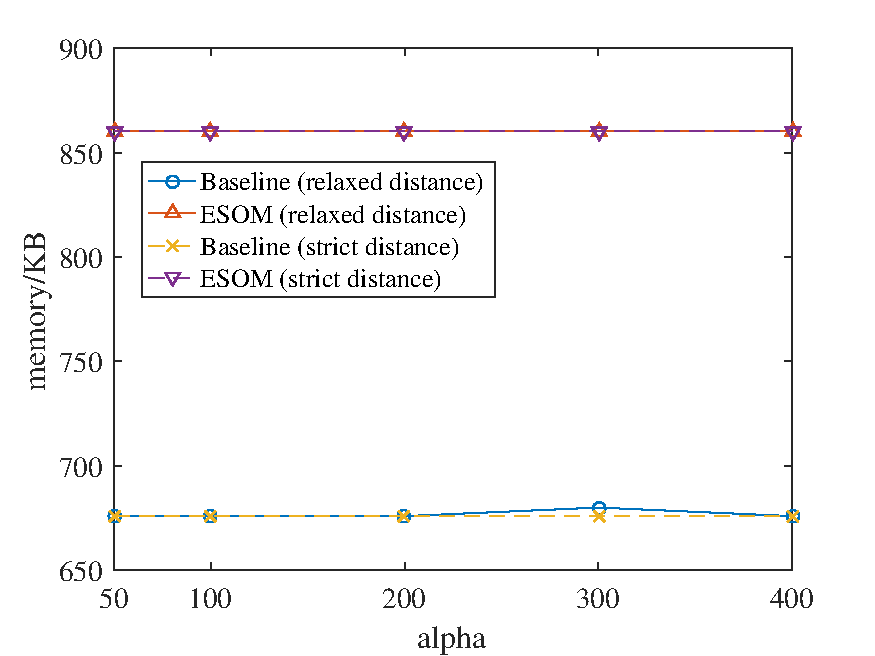
\includegraphics[height=0.18\textheight,width=0.31\textwidth]{f13.pdf}}
	\hspace{1in}
	~~	
	\subfigure[Utility, run time and memory of varying $\delta$]{
		\label{fig:subfig:a} %% label for first subfigure	
		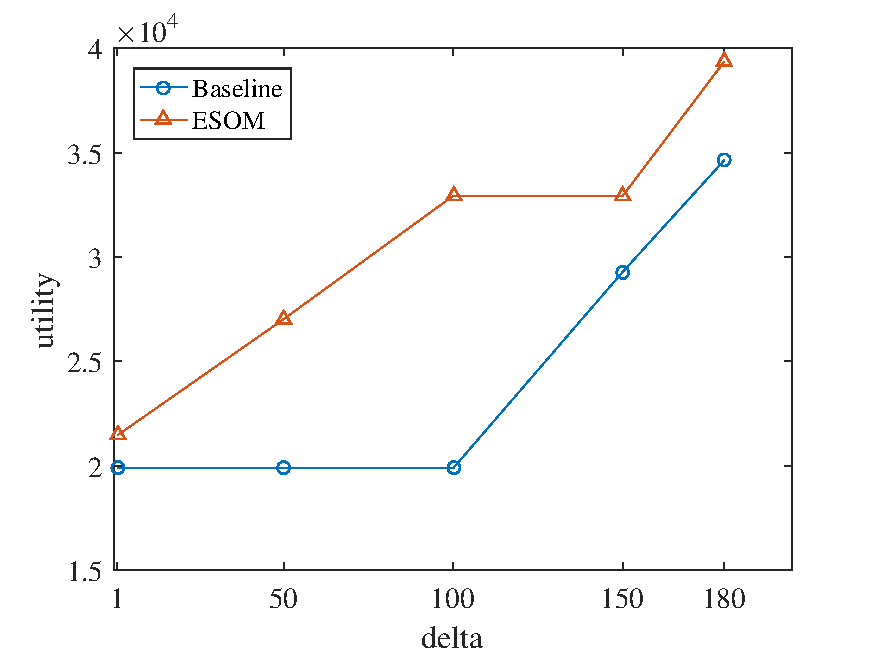
\includegraphics[height=0.18\textheight,width=0.31\textwidth]{f14.pdf}
		\label{fig:subfig:a} %% label for first subfigure	
		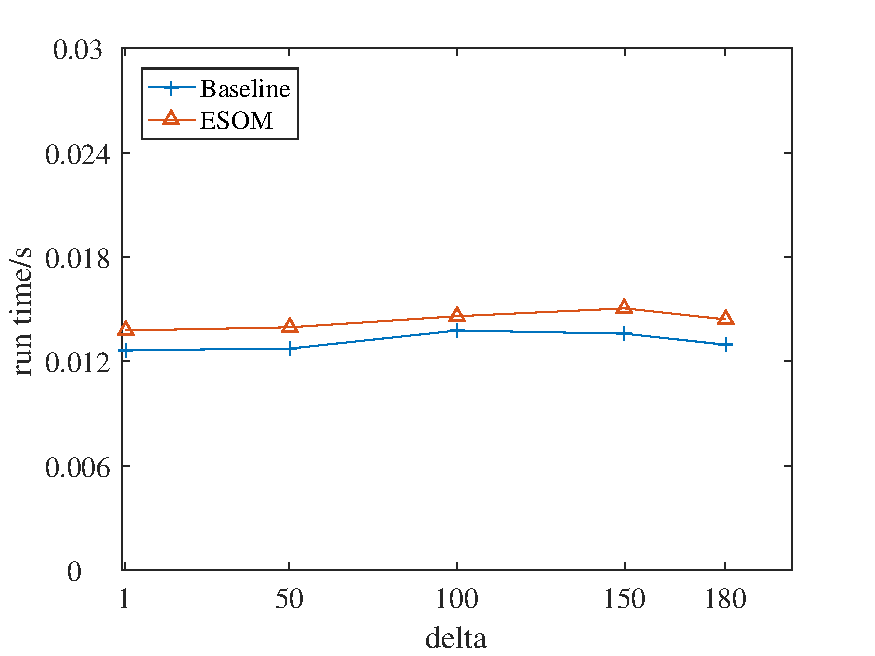
\includegraphics[height=0.18\textheight,width=0.31\textwidth]{f15.pdf}
		\label{fig:subfig:a} %% label for first subfigure	
		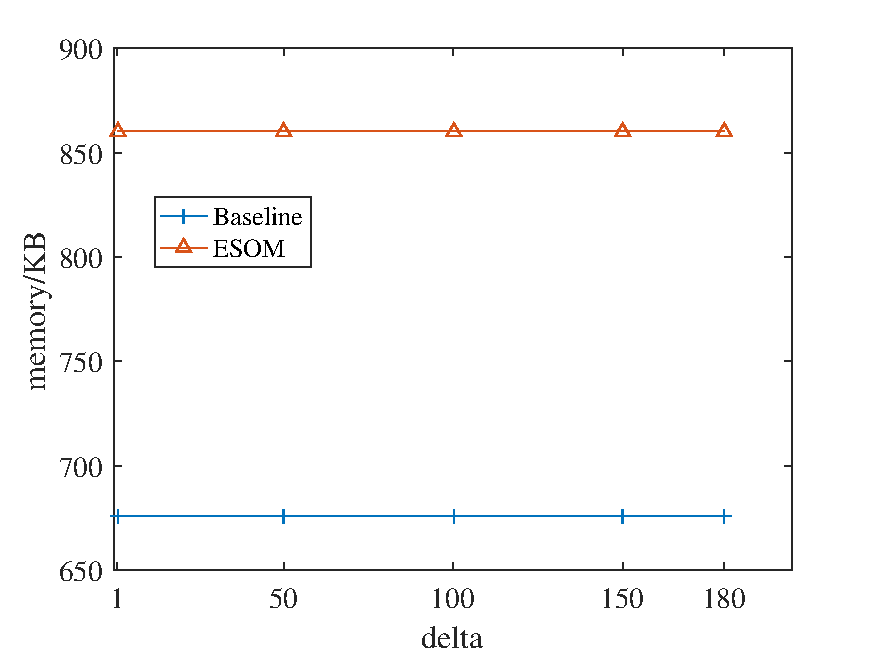
\includegraphics[height=0.18\textheight,width=0.31\textwidth]{f16.pdf}}
	\hspace{1in} 
	~~	
	\caption{Results on varying $\alpha$ and $\delta$}
	\label{fig:subfig} %% label for entire figure
\end{figure*}

\begin{figure*}[htb]
	\centering
	\subfigure[Utility, run time and memory of varying $|W|$]{
		\label{fig:subfig:a} %% label for first subfigure	
		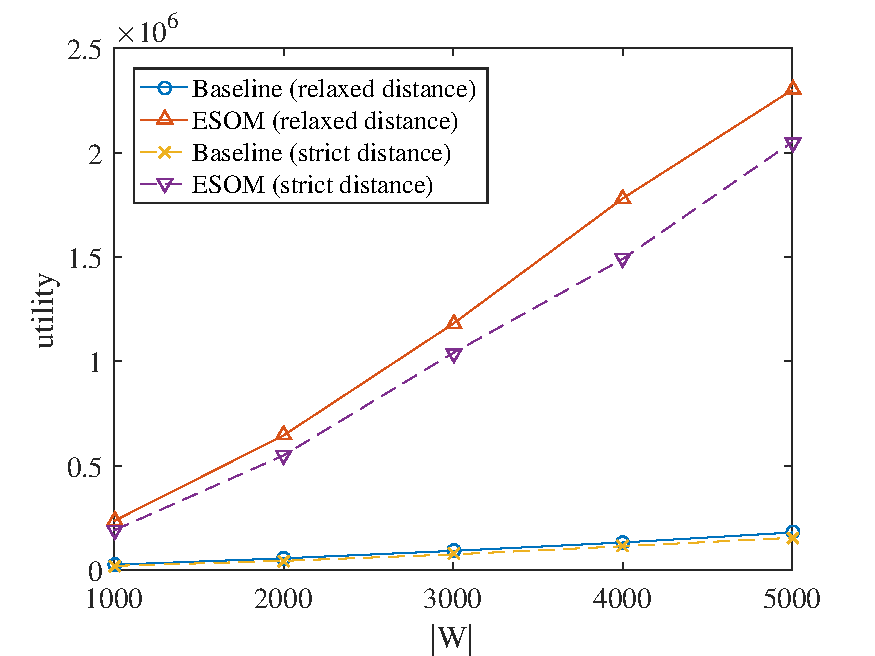
\includegraphics[height=0.18\textheight,width=0.31\textwidth]{f17.pdf}
		\label{fig:subfig:a} %% label for first subfigure	
		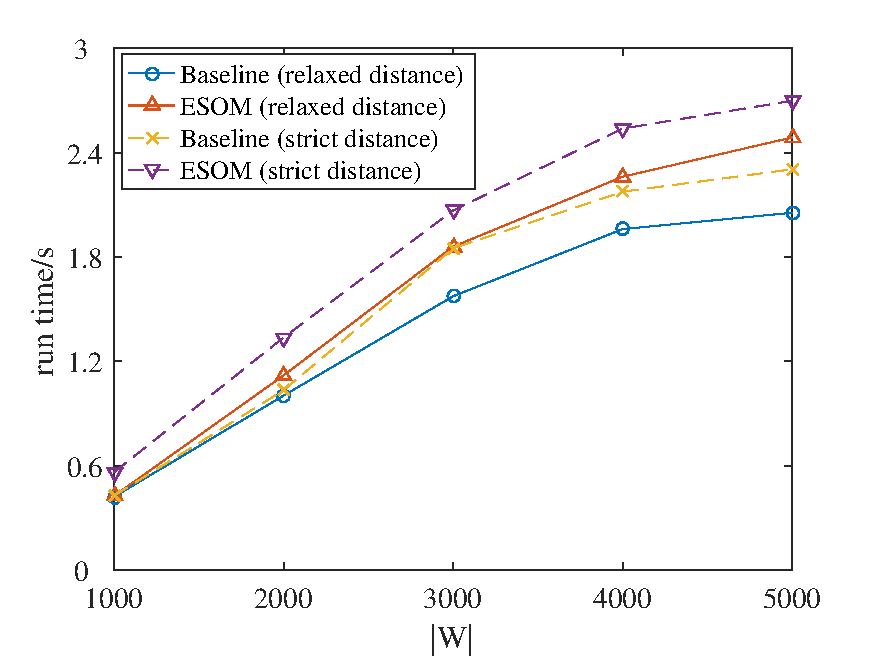
\includegraphics[height=0.18\textheight,width=0.31\textwidth]{f18.pdf}
		\label{fig:subfig:a} %% label for first subfigure	
		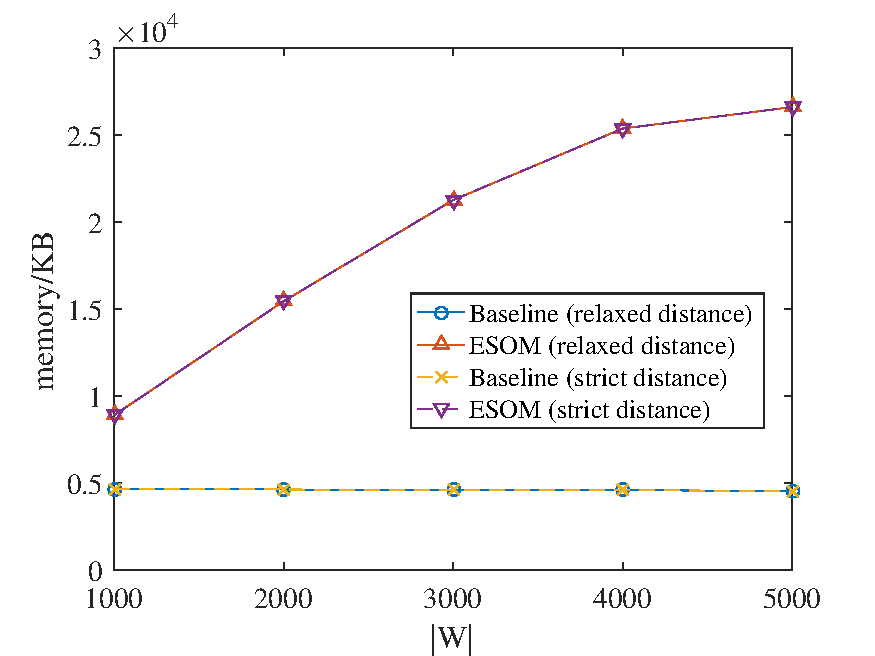
\includegraphics[height=0.18\textheight,width=0.31\textwidth]{f19.pdf}}
	\hspace{1in}
	~~	
	\subfigure[Utility, run time and memory of varying $\alpha$]{
		\label{fig:subfig:a} %% label for first subfigure	
		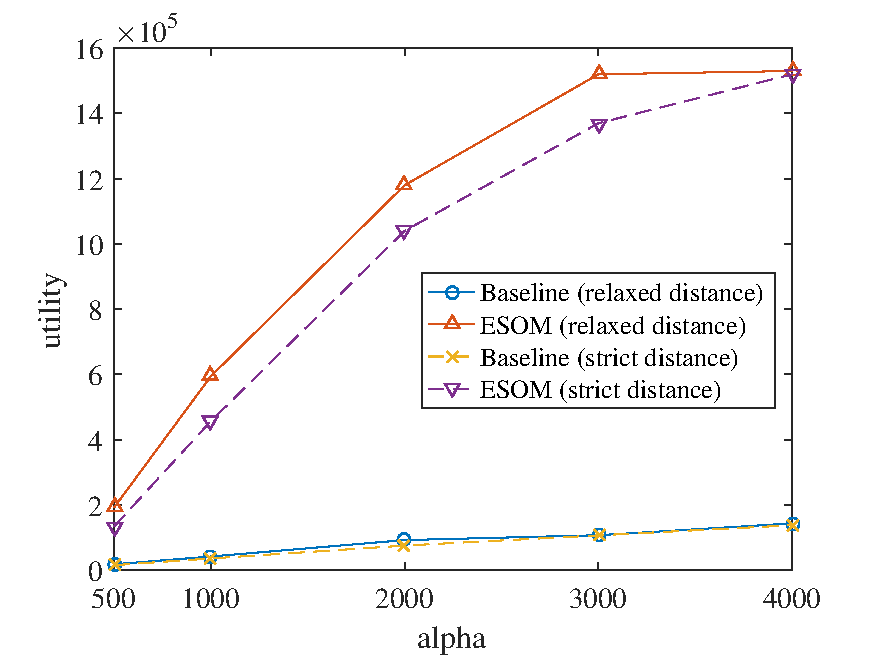
\includegraphics[height=0.18\textheight,width=0.31\textwidth]{f20.pdf}
		\label{fig:subfig:a} %% label for first subfigure	
		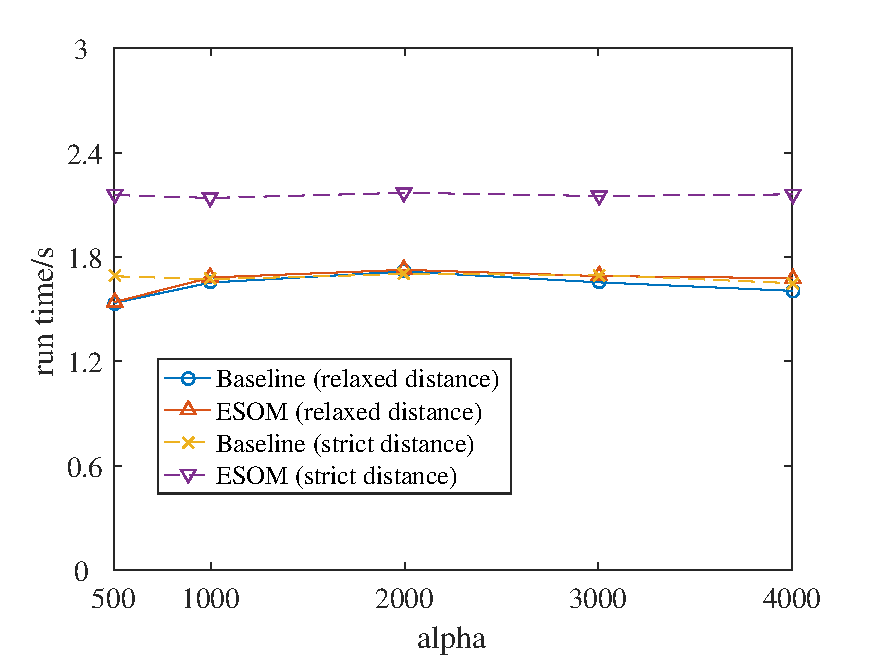
\includegraphics[height=0.18\textheight,width=0.31\textwidth]{f21.pdf}
		\label{fig:subfig:a} %% label for first subfigure	
		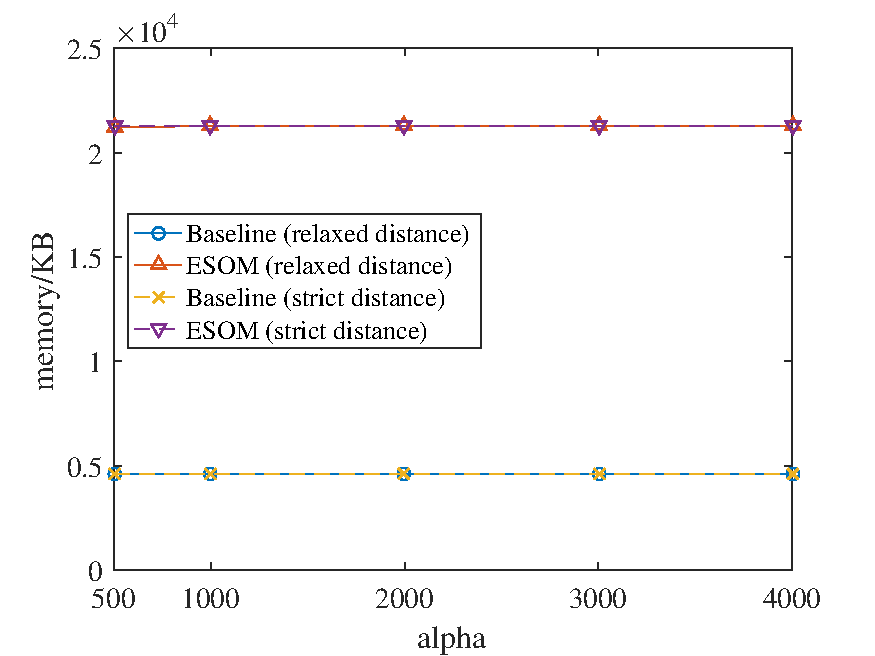
\includegraphics[height=0.18\textheight,width=0.31\textwidth]{f22.pdf}}
	\hspace{1in}
	~~	
	\subfigure[Utility, run time and memory of varying $\delta$]{
		\label{fig:subfig:a} %% label for first subfigure	
		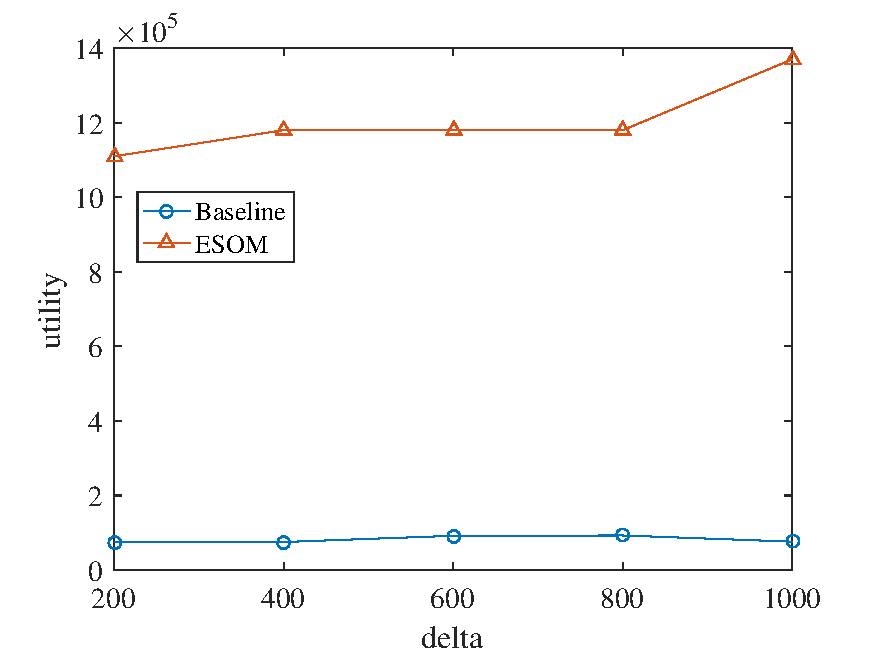
\includegraphics[height=0.18\textheight,width=0.31\textwidth]{f23.pdf}
		\label{fig:subfig:a} %% label for first subfigure	
		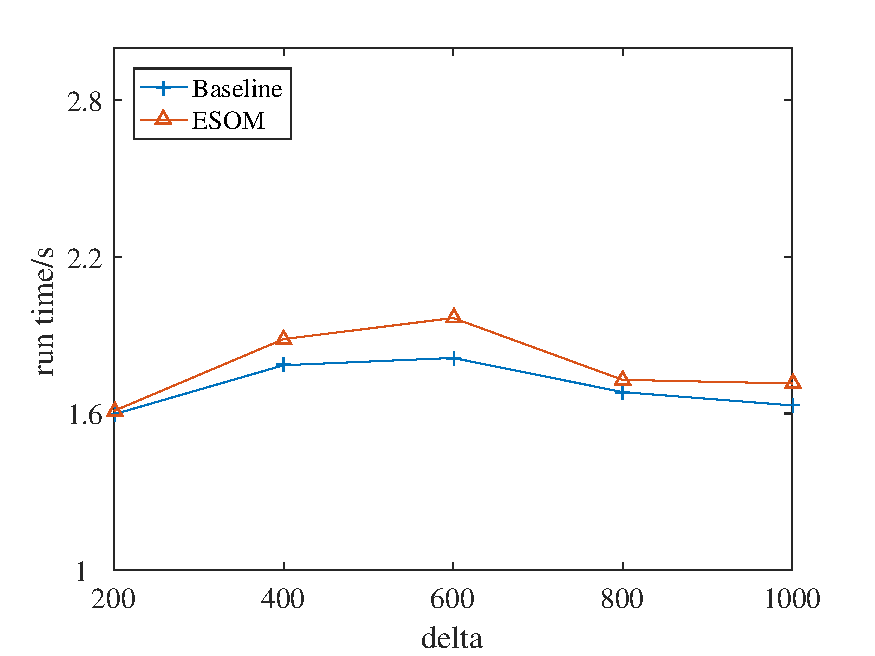
\includegraphics[height=0.18\textheight,width=0.31\textwidth]{f24.pdf}
		\label{fig:subfig:a} %% label for first subfigure	
		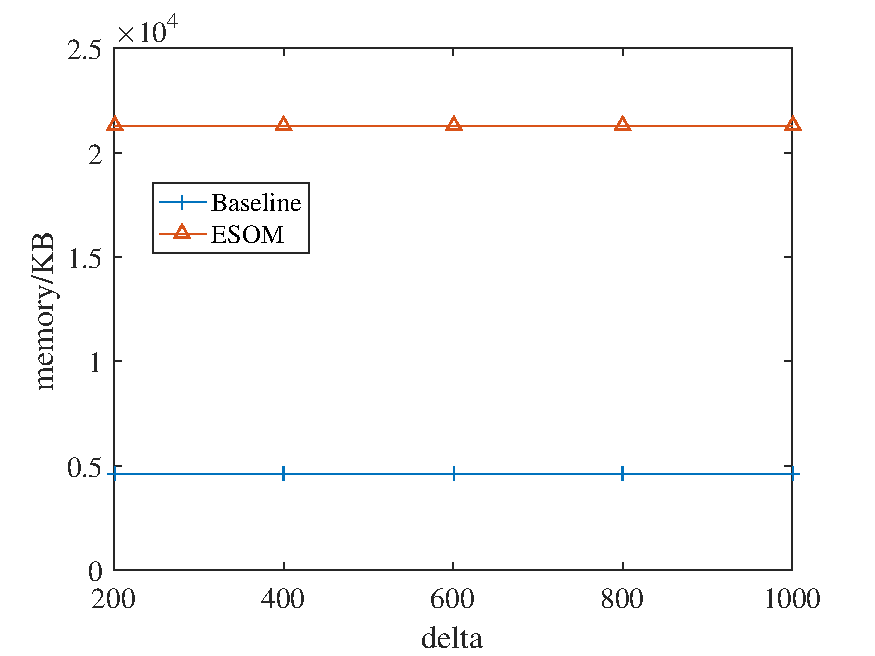
\includegraphics[height=0.18\textheight,width=0.31\textwidth]{f25.pdf}}
	\hspace{1in}
	~~	
	\caption{Results on varying $|W|$, $\alpha$ and $\delta$ on real datasets}
	\label{fig:subfig} %% label for entire figure
\end{figure*}

We use one real dataset, the New York City Taxi and Limousine Commission(NYC TLC) data set\cite{NYCTLC}. NYC TLC is an agency of the New York City government that licenses and regulates the medallion taxis and for-hire vehicle industries. In the NYC TLC dataset, every passenger has a location, a pickup time and trip distance. Since the information of drivers is not given in the dataset, we generate sets of drivers, of whom the locations follow uniform distribution. We also use synthetic datasets for evaluation. We generate the location, utility and appearing time following NYC TLC distribution, too. Statistics of the synthetic datasets are shown in Table 3, where we mark our default settings in bold font. $|T|$ and $|W|$ are the capacities of tasks and workers, $\alpha$ is the threshold of drivers, $\beta$ is the number of parts into which time period is divided, and $\delta$ is the parameter in distance's definition. The distance of $t$ and $w$ is defined as $d(t,w) = \lfloor (|t-w|)/\delta \rfloor \times \delta$ (Here the $\lfloor x \rfloor$ is the integer part of $x$), while Bound is the upper bound of the absolute number of objects' coordinate. Note that here the thresholds of divers are all set as the same number.

We evaluate the Online-Greedy, ESOM algorithms with strict distance and relaxed distance in terms of total utility, running time and memory cost, and study the effect of varying parameters on the algorithms. The algorithms are implemented in Visual Studio Code, and the experiments were performed on a machine with AMD Ryzen 7 PRO 2700U 2.20 GHz CPU and 8GB main memory.


\doublerulesep 0.1pt
\begin{table}[h]
	\begin{footnotesize}
		\caption{Synthetic Dataset}
		\label{tab:1}
		\begin{tabular}{p{2cm}p{6cm}}
			\hline\hline\noalign{\smallskip}
			Factor & \makecell[c]{Setting} \\ 
			\noalign{\smallskip}
			\hline
			$|T|$ & \makecell[c]{1000, 2000, \textbf{3000}, 4000, 5000} \\ 
			$|W|$ & \makecell[c]{1000, 2000, \textbf{3000}, 4000, 5000} \\  
			$|T|\, (|T|=|W|)$ & \makecell[c]{2000, 4000, 6000, 8000, 10000} \\
			$\alpha(Threshold)$ & \makecell[c]{50, 100, \textbf{200}, 300, 400} \\
			$\alpha\, (RealData)$ & \makecell[c]{500, 1000, \textbf{2000}, 3000, 4000} \\
			$\delta(RelaxedDistance)$ & \makecell[c]{1, 50, \textbf{100}, 150, 180} \\
			$\delta\, (RealData)$ & \makecell[c]{200, 400, \textbf{600}, 800, 1000} \\
			$\beta(NumberOfTimePeriods)$ & \makecell[c]{\textbf{50}} \\
			Bound & \makecell[c]{\textbf{3000}} \\
			\hline\hline
		\end{tabular}
	\end{footnotesize}
\end{table}

\noindent{\it B. Experiment Result}


\textbf{Effect of cardinality of both $T$ and $W$}. The results of varying both $|T|$ and $|W|$ are shown in (a) of Figure 2. In terms of total utility, we can first observe that the total utility increases as $|T|$ increases which ought to be as the number of matched pairs increase. Second, we observe that the ESOM algorithm with relaxed distance performs best, followed by the ESOM with strict distance, the Baseline with relaxed distance and the Baseline with strict distance. As for running time, there is little difference between the four algorithms, and at 10000 the ESOM algorithm with strict distance cost a little more than the other algorithms. Finally, as for memory consumption, we can see that it increases as $|T|$ increases. While the ESOM algorithm is less efficient than the Baseline algorithm since they cost more storing space for the substitutable marks.


\textbf{Effect of cardinality of $T$}. The results of varying $|T|$ are shown in (b) of Figure 2. In terms of total utility, we can observe that the value as $|T|$ increases at the first three data points while at the last three ones share the same value which is possibly for their corresponding matching' upper bounds. Also, we see that ESOM algorithm with relaxed distance ranks first among four algorithms. For running time, four algorithms perform similarly and generally it increases as $|T|$ increases . Finally, for memory cost, with low cardinality of $|T|$ ESOM algorithms cost less storing room but when $|T|$ increases they perform worse than baseline algorithms.

\textbf{Effect of cardinality of $W$}. The results of varying $|W|$ are shown in (c) of Figure 2. In terms of total utility, we can first observe that the total utility increases as $|W|$ increases which is ought to be as the number of matched pairs increases. Second, we observe that ESOM algorithm with relaxed distance performs best, followed by ESOM with strict distance, Baseline with relaxed distance and Baseline with strict distance. For running time, four algorithms perform likely and generally it increases as $|W|$ increase. Finally for memory cost, with low cardinality of $|W|$ ESOM algorithms cost less storage but when $|W|$ increases they perform worse than baseline algorithms. when $|W|$ arrives at 4000 the running time decreases, and we think it’s because that the proper distribution structure reduces the number of matched pairs but increases the total utility.

\textbf{Effect of threshold}. The results of varying $\alpha$ are shown in (a) of Figure 3. Concerning total utility, we can observe that it increases with the increment of $alpha$, and the ESOM algorithm with relaxed distance ranks first. As for run time, the varying threshold has no remarkable influence on it. And the four algorithms also show few notable features against each others. For memory cost, ESOM algorithms cost more room, and we can see the change of threshold does not affect on memory cost.

\textbf{Effect of distance's relaxation}. The results of varying Bound are shown in (b) of Figure 3. In terms of total utility, as $\delta$ varies from 1 to 180, the overall profits of ESOM and baseline keep increasing, and at the beginning, the baseline doesn't increase which is probably due to its poor strategy towards the equal distance situation. In the meanwhile the utilities of ESOM keep above the baseline. For running time, the ESOM costs a little more than baseline and the varying of $\delta$ influences little. And for memory cost, the ESOM algorithm costs most storage, and we can see that the varying Bound does not influence memory cost.

\textbf{Real datasets.} We finally present the experiment results on a real dataset. To adapt to the actual scale based on real datasets, we adjust the factor of $\delta$ and $\alpha$ shown in Table 3. The results of varying $|W|$ are shown in (a) of Figure 4. In terms of total utility, it increases as $|W|$ increases, and the ESOM algorithm with relaxed distance ranks first following ESOM with strict distance, Baseline with relaxed distance and Baseline with strict distance. As for run time,
besides natural increment before the point 4000, there is a fall between 4000 and 1000 in $|W|$, which is possible that abundant workers make it easy for tasks to be matched. And also we can observe that ESOM with strict distance costs the most run time. Finally for memory cost, ESOM algorithms cost the most in real datasets. While the results of varying $t$ are shown in (b) of Figure 4. For total utility, it increases as $t$ increases, and we can observe that obviously ESOM algorithms' rates of growth are higher than that of Baseline, and th ESOM with relaxed distance ranks first among four algorithms. As for run time, the ESOM algorithm with strict distance costs the most in contrast to the other three ones. Finally for memory cost, we can observe that ESOM algorithms need more memory space. The results of varying $\delta$ are shown in (c) of Figure 4. The utilities of ESOM are higher than those of baseline, and from 800 to 1000 the ESOM's overall profit increases as that of the baseline keeps flat. As for running time, the ESOM costs more time against the baseline while both are not sensitive to $\delta$'s change. For memory cost, $\delta$ influences little on it.

\noindent{\it C. Experiment Summary}

In terms of total utility scores, the ESOM algorithm with relaxed distance always performs the best among the four algorithms in both synthetic and real datasets. As for running time, with capacity increment, the four algorithms are difference with respect to the number of matched pairs. And in the aspect of memory cost, although the ESOM performs worst for the need of substitutable marks, it's efficient enough to be applied to real-time assignments with low memory cost.

From the Figure 2, Figure 3 and Figure 4 we can see the ESOM algorithm has the advantage on overall profit as either of capacity of tasks or drivers grows and as both of them grow.

\section{Conclusion}

In this paper, we identify a problem with dynamic task assignment, called Revenue-Maximizing Online Stable Matching (RMOSM) Problem. We first analyze its difference with existing task assignment studies that assume the offline scenario, the dynamic bipartite matching problem without stability, or the traditional online stable matching for maximizing revenue. Then, we extend the definition of stability and distance and propose a baseline algorithm called Online-Greedy towards the problem based on traditional algorithms. Although the baseline algorithm can produce a stable matching as an answer, it performs not well enough. To find better solutions, we introduce the concept Substitutable and design a novel algorithm Equation-Substitutable Online Matching (ESOM), which offers more chances to tasks to be assigned, to search for a matching with higher revenue. Finally we conduct experiments that verify the efficiency and effectiveness of the proposed approaches.

\bibliographystyle{unsrt}
\bibliography{ref}

\end{document}
